\documentclass{report}

\usepackage{ressources/packages/miseEnPage}
\usepackage{ressources/vocabulaire/vocabulaire}

\pdfminorversion=4
\usepackage[francais]{babel}
\usepackage[utf8]{inputenc}
\usepackage[T1]{fontenc}
\usepackage{graphicx}
\usepackage{fancyhdr}
\usepackage{pdfpages}
\usepackage{float}
\usepackage{diagbox}
\usepackage[urlcolor=blue, linkcolor=black,linktoc=all, colorlinks=true]{hyperref}
\usepackage[left=2.5cm, right=2.5cm, top=2.5cm, bottom=2.5cm, headheight=15pt]{geometry}
\usepackage[final]{pdfpages}
\usepackage{helvet}
\usepackage{lscape}
\usepackage{wasysym}
\usepackage[multidot]{grffile}

\renewcommand{\familydefault}{\sfdefault}

\makeatletter
\def\@makechapterhead#1{% chapter
  \vspace*{5\p@}
  {
    \parindent \z@ \raggedright \normalfont
    \ifnum \c@secnumdepth >\m@ne
    \huge\bfseries \@chapapp\space \thechapter
    \par\nobreak
    \vskip 5\p@
    \fi
    \interlinepenalty\@M
    \Huge \bfseries #1\par\nobreak
    \vskip 10\p@
    \thispagestyle{fancy}% Permet d'ajouter l'entête de pied de page
  }
}

\def\@schapter#1{
  \if@twocolumn
  \@topnewpage[\@makeschapterhead{#1}]
  \else
  \@makeschapterhead{#1}
  \@afterheading
  \fi
}

\def\@makeschapterhead#1{% chapter*
  \vspace*{5\p@}
  {
    \parindent \z@ \raggedright
    \normalfont
    \interlinepenalty\@M
    \Huge \bfseries  #1\par\nobreak
    \vskip 10\p@
    \thispagestyle{fancy} % Permet d'ajouter l'entête de pied de page
  }
}
\makeatother


\usepackage[utf8]{inputenc}
\usepackage[T1]{fontenc}
\usepackage[francais]{babel}
\frenchbsetup{StandardLists=true}
\usepackage{enumitem}
\usepackage{graphicx, titlesec}

\begin{document}
\lstset{ %
  backgroundcolor=\color{white},   % choose the background color; you must add \usepackage{color} or \usepackage{xcolor}
  basicstyle=\footnotesize,        % the size of the fonts that are used for the code
  breakatwhitespace=false,         % sets if automatic breaks should only happen at whitespace
  breaklines=true,                 % sets automatic line breaking
  captionpos=b,                    % sets the caption-position to bottom
  commentstyle=\color{mygreen},    % comment style
  deletekeywords={...},            % if you want to delete keywords from the given language
  escapeinside={\%*}{*)},          % if you want to add LaTeX within your code
  extendedchars=true,              % lets you use non-ASCII characters; for 8-bits encodings only, does not work with UTF-8
  frame=single,                    % adds a frame around the code
  keepspaces=true,                 % keeps spaces in text, useful for keeping indentation of code (possibly needs columns=flexible)
  keywordstyle=\color{blue},       % keyword style
  language=C++,                    % the language of the code
  morekeywords={*,...},            % if you want to add more keywords to the set
  numbers=left,                    % where to put the line-numbers; possible values are (none, left, right)
  numbersep=5pt,                   % how far the line-numbers are from the code
  numberstyle=\tiny\color{mygray}, % the style that is used for the line-numbers
  rulecolor=\color{black},         % if not set, the frame-color may be changed on line-breaks within not-black text (e.g. comments (green here))
  showspaces=false,                % show spaces everywhere adding particular underscores; it overrides 'showstringspaces'
  showstringspaces=false,          % underline spaces within strings only
  showtabs=false,                  % show tabs within strings adding particular underscores
  stepnumber=2,                    % the step between two line-numbers. If it's 1, each line will be numbered
  stringstyle=\color{mymauve},     % string literal style
  tabsize=2,                       % sets default tabsize to 2 spaces
  title=\lstname                   % show the filename of files included with \lstinputlisting; also try caption instead of title
} 
\lstset{
language=Java,
basicstyle=\normalsize, % ou ça==> basicstyle=\scriptsize,
upquote=true,
aboveskip={1.5\baselineskip},
columns=fullflexible,
showstringspaces=false,
extendedchars=true,
breaklines=true,
showtabs=false,
showspaces=false,
showstringspaces=false,
identifierstyle=\ttfamily,
keywordstyle=\color[rgb]{0,0,1},
commentstyle=\color[rgb]{0.133,0.545,0.133},
stringstyle=\color[rgb]{0.627,0.126,0.941},
}
\couverture{}
\pagestyle{pageNormale}

\setcounter{page}{1}
\tableofcontents{}
\chapter{Introduction}
	\section{Introduction}

Notre programme sera une plateforme permettant la gestion de portefeuille. Pour cela, nous offrirons la possibilité à l’utilisateur pour chaque actif disponible divers outils d’analyse technique. \\ \\


Notre programme sera une plateforme permettant la gestion de portefeuille. Pour cela, nous offrirons la possibilité à l’utilisateur pour chaque actif disponible divers outils d’analyse technique. A partir de cela, nous lui fournirons un conseil concernant l’actif sélectionné (signal de vente, signal d’achat, …). \\ \\
	Nous lui proposerons également une analyse plus pointue qui lui permettra de regarder le comportement de ses actifs en tant que portefeuille par exemple avec la méthode de Black-Scholes ou Markowitz. \\ \\
	La finalité du projet serait de réaliser un jeu en réseau qui permettrait à chaque joueur de créer son portefeuille, de voir son évolution et de la comparer aux autres joueurs : le gagnant sera le joueur le plus riche (ou le moins pauvre). 


Notre projet va donc se découper en trois phases principales : 
\begin{itemize}
\item La première consistera à récupérer les données des cours et les stocker par l’intermédiaire d’une base de données.
\item La deuxième étape sera le traitement de ces données (outils d’analyse technique).
\item Enfin, nous proposerons à l’utilisateur d'afficher des indicateurs sur les historiques mais également de visualiser son portefeuille. 
\end{itemize}



\section{Base de données}
Gestion des différents cours des actifs (Nom, valeur à l’ouverture, à la clôture, la plus haute et la plus basse pendant la séance). \\ \\ 
Deux options pour la récupération des données : soit on les stocke dans une base de donnée statique, c’est-à-dire, nous aurons récupéré les cours pour une certaine durée. Nous placerons le début du jeu dans le passé, de manière à pouvoir constater les gains ou pertes du joueur. La deuxième méthode pour gérer nos données, consisterait à actualiser notre base de données à la demande du joueur en allant chercher les données sur un serveur web. 

\section{Gestion des actifs}
Pour chaque actif nous proposerons une analyse des divers cours que nous aurons dans notre base de données. Pour cela nous utiliserons des outils d’analyse technique. \\ \\
A la fin de l’analyse, nous proposerons un avis sur l’actif. 

\section{Indicateurs}
Chaque utilisateur aura la possibilité de consulter l’ensemble de son portefeuille. Pour cela un descriptif lui sera affiché avec les fonctionnalités suivantes : détails (composition du portefeuille, liste des actifs), performance (rendement) et répartition par actifs par types. \\ \\
Chaque utilisateur aura la possibilité de consulter l’ensemble de son portefeuille. Pour cela un descriptif lui sera affiché avec les fonctionnalités suivantes : détails (composition du portefeuille, liste des actifs), performance (rendement) et répartition par actifs par types. \\ \\
Ensuite pour chaque action, il sera possible de visualiser la valeur du cours, sa variation et son volume, un graphique et plusieurs possibilités d’indicateurs. 


\subsection{Différentes versions envisagées}
Pour réaliser ce projet, nous avons choisi de nous fixer divers objectifs à atteindre. Chacun de ces objectifs correspond à une nouvelle qui sera pour la première une version très simplifiée du projet final à laquelle nous ajouterons les différents éléments au fur et à mesure. \\ 
\section{Version 1}
Dans la première version, le joueur aura la possibilité de s'ajouter à la liste des joueurs, d'ajouter lui même les actions qui constitueront la bourse, d'acheter ou de vendre une action et de voir le contenu de portefeuille. \\ \\
Cette première version nous permettra d'avoir la base de notre projet. 

\section{Version 2}
Dans la deuxième version, nous allons ajouter la dimension base de données à notre projet. C'est-à-dire, que toutes les données qui seront ajoutées au fur et à mesure du jeu ne seront pas perdus comme dans la version précédente quand le jeu se fermera. \\ \\
Ensuite, le joueur n'aura plus la possibilité de choisir les actions et leur valeur lui-même mais il y aura une table qui regroupera les différentes actions qui sont possibles pour le joueur. Nous pourrons ainsi stocker l'historique de chacun des cours également (nous nous contenterons dans un premier temps des actions du CAC 40). 

\section{Version 3}
Dans cette version, nous allons rajouter le téléchargement des cours via l'API Yahoo. A chaque lancement du jeu, nous mettrons à jour la base de données depuis la dernière connexion pour compléter les données manquantes. Nous aurons ainsi un historique complet pour les cours de nos actions. 

\section{Version 4}
Nous allons pour ce nouveau objectif rajouter le tracé des cours. Le joueur pourra avoir une représentation graphique de l'évolution des cours depuis l'historique que nous trouverons dans la base de données remplies précédemment. 

\section{Version 5}
Nous choisirons plusieurs indicateurs techniques que nous mettrons à la disponibilité de chaque joueur. Nous essaierons de lui livrer un conseil à partir de chacun de nos indicateurs (signal de vente, signal d'achat etc). 

\section{Version 6}
Dans cette partie, nous améliorerons la qualité des informations fournies au joueur. Nous  
allons essayer de lui proposer une vision de son portefeuille plus détaillés avec un graphique représentant l'évolution de la valeur de son portefeuille, plus de possibilités en terme d'actions : en essayant d'en augmenter le nombre, de les classifier par secteur, ...

\section{Version 7}
Nous allons pour cette partie développer un véritable mode multijoueur sur un seul ordinateur. Jusqu'à présent le joueur pouvait s'ajouter à la liste des joueurs mais ne devait pas s'identifier par le biais d'un mot de passe ce qui sera mis en place. De plus, il pourra consulter le classement des autres joueurs. 

\section{Version 8}
Dans cette ultime version, nous pourrons nous connecter à notre base de données à distance et ainsi nous pourrons joueur sur plusieurs machines à notre jeu. 
	
	\textcolor{red}{\LARGE{\textbf{Ajouter le début du prérapport : besoin et exigences, versions}}}


\chapter{Techniques utilisées}
Une partie important de notre projet de fin d'étude était de savoir quelles techniques utiliser afin de répondre à nos besoins et exigences. Nous avons choisi de créer un site Internet en utilisant le langage Java et pour cela, l'environnement Eclipse avec un Web Dynamic Project s'y prete bien.
Dans cette partie nous allons donc développer les différents points informatiques techniques que nous avons abordé et nous détaillerons les choix que nous avons fait pour notre application.
	\section{Le modèle MVC et l'environnement Java EE}

%%%%%%%%%%%%%%%%%%%%%%%%%%%%%%%%%%%%%%%%%%%%%%%%%%%%%%%%%%
%----------------------MVC-------------------------------%
%%%%%%%%%%%%%%%%%%%%%%%%%%%%%%%%%%%%%%%%%%%%%%%%%%%%%%%%%%
\subsection{Architecture Modèle-Vue-Contrôleur}
Etant donné le fait que nous avons choisi de faire une application interactive, nous avons utilisé l'architecture logicielle \textbf{MVC}. Ainsi, les problématiques liées aux composantes de notre application sont bien séparées :
\begin{description}
 \item[Le modèle :] notre code Java qui modélise les données et qui sera relié à une base de données pour stocker diverses informations. C'est le coeur du programme.
 \item[La vue :] l'interface homme-machine qui sera sous forme d'un site Web.
 \item[Le contrôleur :] la partie de notre code qui fait le lien entre le modèle et la vue. Il agit en fonction de ce que l'utilisateur demande à la vue. Il est chargé de de chaque côté et les transmets à l'un et l'autre comme le montre le schéma ci-dessous.\\
\end{description}

Le schéma suivant présente les intéractions entre les trois entités de notre architecture logicielle.
\begin{figure}[H]
  \center
  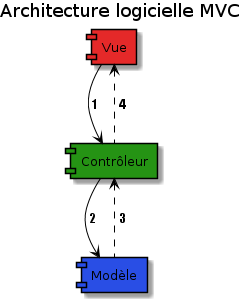
\includegraphics[scale=0.6]{../graph/MVC.png} \\
  \caption{Structure MVC}
\end{figure}

\begin{enumerate}
 \item L'utilisateur intéragi avec la vue (le site Web) et lance une action du contrôleur qui reçoit les informations.
 \item Le contrôleur agit alors en conséquence en envoyant des informations au modèle.
 \item Le modèle traite les informations puis renvoie le résultat de son action au contrôleur et des données dans certains cas.
 \item Le contrôleur fait un compte rendu à l'utilisateur en mettant à jour la vue.
\end{enumerate}

Nous allons voir dans la partie suivante comment sont implémentées nos différentes composantes.

%%%%%%%%%%%%%%%%%%%%%%%%%%%%%%%%%%%%%%%%%%%%%%%%%%%%%%%%%%
%----------------------JEE-------------------------------%
%%%%%%%%%%%%%%%%%%%%%%%%%%%%%%%%%%%%%%%%%%%%%%%%%%%%%%%%%%
\subsection{Environnement Java EE}
L'environnement de développement Java EE (Java Enterprise Edition) est une extension de la plateforme standard Java. On y compte davantage de bibliothèques. Le principal objectif de Java EE est de faciliter le développement d'applications web. Il permet notamment de créer des sites dynamiques.\\

De manière générale, un échange dynamique se présente ainsi : un client est sur le navigateur de son ordinateur et lui demande une page. Derrière, un serveur va générer la page puis l'envoyer au navigateur du client.
La communication entre le client et le serveur se fait grâce au protocole HTTP sous forme de requête du client vers l'utilisateur et de réponse au retour.
Un navigateur ne fait rien d'autre que traduire/interpréter des informations qui lui sont envoyées sous forme HTML, CSS et Javascript. Le serveur ne devra donc renvoyer des informations qu'à l'aide de ces technologies.
De même, le serveur de son côté utilise des technologies propres à lui qui lui permettent d'analyser les données reçues, de les transformer, de les enregistrer dans une base de données, etc... Finalement, il doit générer des pages web à envoyer au client après avoir réaliser les traitements nécessaires.\\

D'autres technologies que Java EE permettent de traiter les informations sur le serveur comme PHP, .NET ou encore Django, mais nous avons préférer utiliser un environnement connu et déjà utilisé lors d'autres projets. Ainsi nous avons pu gagner un peu de temps et nous pencher sur d'autres problématiques. De plus, nous souhaitions utiliser le langage Java et cette technologie nous le permet.

Un avantage de Java EE est qu'il a été créé notamment pour faciliter le travail en équie sur un même projet. En effet, l'application est formée de plusieurs couches.\\

\subsubsection{Mise en place sous Eclipse}
Pour créer notre application web avec Java EE nous avons besoin d'un \textit{Environnement de Développement Intégré} (IDE) qui est un logiciel facilitant le développement de l'application. Nous avons choisi d'utiliser l'IDE Eclipse qui nous était déjà familier et car il est gratuit, puissant, libre et multiplateforme.\\
Un tel logiciel a différents avantages comme par exemple :
\begin{itemize}
 \item Une interface graphique avec une hiérarchie permettant de visualiser l'architecture de l'application
 \item L'intégration des outils nécessaires au développement de l'application.
 \item La possibilité de paramétrer facilement les composants de l'application.
 \item L'aide à l'écriture du code et même la génération automatique de certaines fonctions (exemple : les getters et setters).
 \item Un outil pour déboguer facilement.
\end{itemize}

On utilise donc la version d'Eclipse adéquate disponible sur le site officiel :
\begin{figure}[H]
  \center
  
\includegraphics[scale=0.5]{../graph/eclipse.png} \\
  \caption{Eclipse IDE for Java EE Developers - \url{https://eclipse.org/downloads/}}
\end{figure}

Une fois qu'Eclipse est installé, il est nécessaire de mettre en place un serveur d'applications. Nous avons utilisé Tomcat car il est libre, gratuit, multiplateforme et léger. Il est suffisant pour notre application.

\paragraph{Le serveur Apache Tomcat}
Apache Tomcat est un conteneur web libre de servlets et JSP Java EE. Nous verrons dans les parties suivantes ce que sont les servlets et les JSP. Il permet notammement l'utilisation des servlets et des JSP (JavaServer Pages).
Tomcat est un serveur HTTP avant tout. Il est écrit en Java ce qui permet de l'utiliser sur n'importe quelle système d'exploitation via la machine virtuelle Java.\\
\begin{figure}[H]
  \center
  
\includegraphics[scale=0.3]{../graph/apache.png} \\
  \caption{Apache Tomcat - \url{http://tomcat.apache.org/index.html}}
\end{figure}
En réalité, ce n'est pas un vrai serveur d'application mais un serveur web assemblé à un conteneur web. Dans notre projet, nous utilisons la dernière version d'Apache Tomcat 8.0 qui est suport de Java 7 et possède d'autres avantages dont nous avons besoin.\\

\paragraph{Dynamic Web Project}
Maintenant que le serveur Tomcat est ajouté, on peut créer le projet dans Eclipse. On crée un Dynamic Web Projet qui nous permettra de faire notre application.
Le schéma suivant donne la structure des fichiers de notre dossier projet :\\
\begin{figure}[H]
  \center
  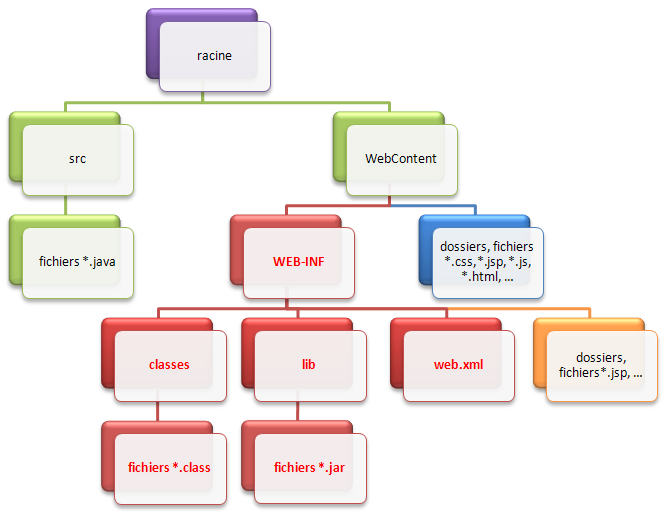
\includegraphics[scale=0.5]{../graph/schemaProjetDynamic.png} \\
  \caption{Structure des fichiers d'une application web JSP/Servlet sous Eclipse (Java EE) - \url{https://openclassrooms.com/courses/creez-votre-application-web-avec-java-ee/outils-et-environnement-de-developpement}}
\end{figure}
Quelques remarques sur le schéma précédent :
\begin{itemize}
 \item Le dossier src : c'est ici que se trouvent les packages Java et notamment les packages du modèle et du contrôleur.
 \item Le dossier WEB-INF : il est spécial et essentiel au bon fonctionnement de l'application. Il contient le fichier web.xml qui configure l'application, un dossier nommé classes qui contient les classes Java compilées et un dossier lib contenant les bibliothèques supplémentaires (.jar). Cette structure du dossier WEB-INF doit impérativement être comme ci-dessus.
 \item Les fichiers et dossiers publics sont placés dans le WebContent (en bleu) et les privés dans le WEB-INF. Cette notion de public/privé servira notamment lorsque l'on voudra bloquer l'accès à certaines pages.
 \item Le dossier WebContent est propre à Eclipse et n'est pas un dossier nécessaire à l'origine.
\end{itemize}
Enfin, il est important de préciser que si l'application n'est pas strucutrée de cette manière alors le serveur d'applications ne sera pas capable de la déployer et ainsi elle ne pourra pas fonctionner correctement.\\


Le projet est maitenant ouvert et il est alors possible de créer une première page web. Si l'on voulait créer une simple page web statique il suffirait de créer une fichier HTML dans le dossier WebContent. Pour créer des pages dynamiques on va avoir recours aux servlets et aux Java Server Pages décrites dans ce qui suit.


\subsubsection{Les servlets}
Les servlets sont des classes implémentées en Java qui permettent de rendre
dynamique une page HTML. Elles utilisent l'API Java Servlet qui correspond au
package javax.servlet.\\

Si on repart du schéma suivant, on reprend le mécanisme existant entre le client
et le serveur HTTP : le client envoie une requête HTTP au serveur et ce dernier
lui retourne une réponse.\\
\begin{figure}[H]
  \center
  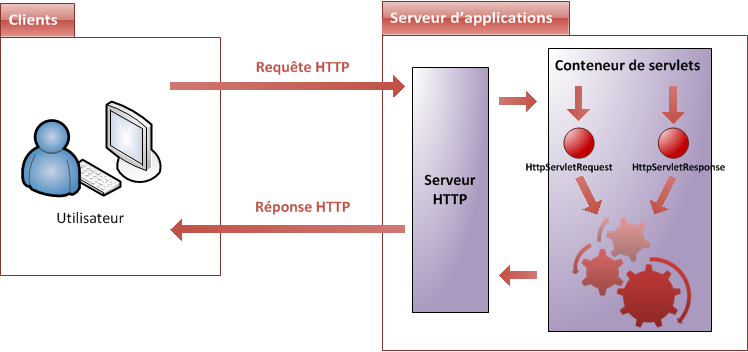
\includegraphics[scale=0.5]{../graph/serveurclient.png} \\
  \caption{Schéma serveur client HTTP - https://openclassrooms.com/courses/creez-votre-application-web-avec-java-ee/la-servlet}
\end{figure}

Tout l'intérêt de l'utilisation des servlets réside dans le fait qu'il devient
alors possible de maîtriser le traitement des requêtes mais surtout de personnaliser
les réponses HTTP qui sont faites au client.\\

Ainsi, dans la plus part des cas, le fonctionnement d'une servlet peut se résumer
au fait que c'est une classe Java qui reçoit une requête HTTP envoyée depuis un
navigateur par un client et lui renvoie une réponse HTTP.\\

L'ensemble des servlets est appelé conteneur de servlets ou conteneur web.

Lors de l'implémentation d'une servlet en Java, il faut créer une classe qui hérite
de la classe abstraite HttpServlet et pour cette raison elle doit implémenter à
minima l'un des trois méthodes suivantes :
\begin{itemize}
 \item doGet() : gère la méthode GET 
 \item doPost() :
 \item doHead() :
\end{itemize}


parler du XML (un pour chaque servlet)




En effet, une page HTML est statique et si on souhaite la rendre dynamique
A titre d'exemple, Ainsi, les servlets seront assimilées au contrôleur de notre
archicture MVC (et les pages JSP à la vue).\\

\subsubsection{Les JSP (Java Server Pages)}
Une Java Server Page (on utilisera le terme de JSP par la suite) est un document texte
qui peut contenir des balises HTML mais également des balises permettant d'inclure
du code Java. Le langage utilisé dans les JSP permet aussi l'utilisation d'autres
technologies comme XML, les servlets, le CSS... et ce dans un seul et unique fichier
ce qui rend les rend d'autant plus intéressante.\\

On utilise des JSP car cela simplifie l'utilisation des technologies servlets.
En effet, écrire une page web en Java peut vite devenir pénible. Les JSP permettent
donc d'utiliser la technologie des servlet d'une manière simplifiée puisqu'on peut
écrire une page HTML de manière classique.\\

D'autre part, on les utilise afin de respecter la structure MVC puisque cela permet
de retirer des servlets la partie 'vue' et de n'y laisser que la partie 'contrôleur'.
De même on sépare la vue du modèle puisque il peut se trouver au milieu des servlets
du code métier. Ainsi, la servlet est le contrôleur qui relie la vue (JSP) au modèle.
Tout ceci respectant bien l'architecture MVC.\\


L'avantage de l'utilisation des JSP est que les pages sont exécutées 
par un serveur et ainsi on peut avoir une page dynamique contrairement aux pages
HTML basiques.\\
La page étant alors dynamique, on peut faire varier l'affichage de la page et
avoir une interaction avec l'utilisateur.\\
Les JSP 

FAIRE EXEMMLE MVC avec Joueur

	
	\section{Les pages Web}
biblio
https://www.w3.org/TR/html5/ \\
https://fr.wikipedia.org/wiki/HTML5 \\
https://fr.wikipedia.org/wiki/Hypertext\_Markup\_Language

http://adiguba.developpez.com/tutoriels/j2ee/jsp/jstl/\#L1.1
http://www.objis.com/formation-java/tutoriel-jstl-installation-jakarta-taglib.html

%%%%%%%%%%%%%%%%%%%%%%%%%%%%%%%%%%%%%%%%%%%%%%%%%%%%%%%%%%
%----------------------HTML/CSS--------------------------%
%%%%%%%%%%%%%%%%%%%%%%%%%%%%%%%%%%%%%%%%%%%%%%%%%%%%%%%%%%
\subsection{HTML, CSS et JavaScript}
Pour créer nos pages web nous allons utiliser le langage HTML5. Généralement, lorsque l'on parle d'HTML5 cela comprend également le CSS3 et le JavaScript, qui forment à eux trois des technologies Web permettant de développer des applications.
\begin{figure}[H]
  \center
  
\includegraphics[scale=0.6]{../graph/html5.png} \\
  \caption{ \url{https://fr.wikipedia.org/wiki/HTML5}}
\end{figure}

Le HTML est un langage de balisage qui permet d'écrire de l'hypertexte, ces balises permettent de structurer les pages Web et on peut également y inclure du contenu multimédia (images notamment). On utilise en parallèle le CSS afin de faire un format uniforme qui est fonction le plus souvent des balises. Ainsi, la feuille de style (.css) qui est créée peut être appliquée à toutes les pages Web et on obtient alors un site avec un format homogène et ce en ayant un code léger puisqu'on n'a pas besoin de s'occuper du format au sein de chaque page mais seulement de faire attention aux balises utilisées.\\

Par ailleurs, on a dit que l'on pouvait intégrer du code écrit en JavaScript dans les pages HTML. Cela peut permette notamment de personnaliser la page et de réagir à certaines actions de l'utilisateur. Par exemple, il existe un évènement 'OnMouseOver' qui se déclanche lorsque l'on passe la souris sur un élément de la page, on peut alors choisir la réaction que va avoir la page Web. Un exemple simple est lorsque l'on passe sur une image, elle grossit. \\

JavaScript permet également de faire des choses comme le calendrier que nous allons utiliser dans notre application. En effet, nous avons besoin de faire choisir à l'utilisateur des dates, pour qu'il saisisse une date valide directement, nous avons préféré lui proposer un calendrier. Pour cela, Javascript est un bon outil. Dans l'exemple qui suit, l'utilisateur cliquera dans la case blanche réservée à la saisie d'une date et verra s'afficher le calendrier en-dessous. On peut remarquer par ailleurs que le calendrier est personnalisé : nous avons utilisé le langage CSS afin d'utiliser le même format pour le calendrier que pour les pages.
\begin{figure}[H]
  \center
  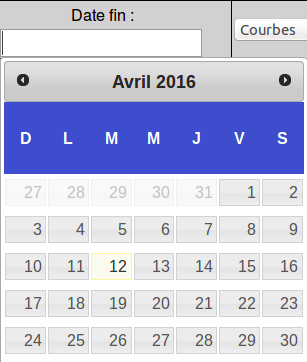
\includegraphics[scale=0.5]{../graph/JavaScriptCalendrier.png} \\
  \caption{Exemple d'utilisation de JavaScript pour afficher des éléments intéractifs dans la page Web.}
\end{figure}

JavaScript nous servira également lorsque nous voudrons ajouter des graphiques à nos pages Webs et cela en utilisant un API Google Chart qui sera intégrée à l'application via le langage JavaScript.

%%%%%%%%%%%%%%%%%%%%%%%%%%%%%%%%%%%%%%%%%%%%%%%%%%%%%%%%%%
%----------------------JSTL------------------------------%
%%%%%%%%%%%%%%%%%%%%%%%%%%%%%%%%%%%%%%%%%%%%%%%%%%%%%%%%%%
\subsection{La libraire JSTL}
Comme nous l'avons vu précédemment, nous utilisons des pages JSP qui permettent de créer des pages Web dynamiques et ce notamment en y incorporant du code Java. Afin de faciliter l'écriture des JSP et aussi de les rendre plus 'propres', on peut utiliser des \textbf{tags}. La librairie JSTL (Java Standard Tags Librairy) procure un certain nombre de tags prédéfinis.\\

On intègre à nos JSP cette librairie avec la ligne suivante en tout début de page (avant les balises <HTML>). Cela permet alors d'utiliser les tags (simples) de la librairie. Si on veut utiliser d'autres tags de format ou fonctions, il faut intégrer les deux lignes suivantes.
\begin{lstlisting}[language=XML]
<%@ taglib uri="http://java.sun.com/jsp/jstl/core" prefix="c" %>
<%@ taglib uri="http://java.sun.com/jsp/jstl/functions" prefix="fn" %>
<%@ taglib uri="http://java.sun.com/jsp/jstl/fmt" prefix="fmt" %>
\end{lstlisting}  

Il existe tout un ensemble de balises, si l'on cite les plus importantes, on aura :\\

\noindent
\begin{tabular}{|l|l|}
  \hline
      <c:\textbf{set} var="un" value="1"/> 		& Déclarer des variables. \\ 
  \hline 
      <c:\textbf{import} url="/inc/menu.jsp" /> 	& Importer une autre page JSP. \\
  \hline 
      <c:\textbf{if} test="boolean"></c:\textbf{if}> 	& Exécuter un test. \\
  \hline        					    
      <c:\textbf{forEach} var="var" items="tableau" >> 	& Exécuter une boucle sur un tableau ou une autre structure, \\
      </c:\textbf{forEach}				& la variable var est une sorte d'itérateurs sur la structure. \\
  \hline        					    
\end{tabular}

	
	\section{La base de données}

%%%%%%%%%%%%%%%%%%%%%%%%%%%%%%%%%%%%%%%%%%%%%%%%%%%%%%%%%%
%----------------------MySQL-----------------------------%
%%%%%%%%%%%%%%%%%%%%%%%%%%%%%%%%%%%%%%%%%%%%%%%%%%%%%%%%%%
\subsection{MySQL}

\subsubsection{Présentation}
MySQL est un système de gestion de bases de données (SGDB) relationnelles. Ce logiciel étant libre et open source, il est accessible à tout le monde et gratuitement dans la plupart des cas.
Il utilise le langage SQL (Stuctured Query Language) pour les requêtes.

\subsubsection{Mise en place}
La mise en place de MySQL est assez simple. Il suffit de télécharger MySQL pour la version du système d'exploitation utilisé. On aura alors accès à un environnement en local dans lequel il est possible de créer des bases de données.\\

On fait maintenant l'hypothèse que l'on utilise Linux. On pourra alors créer notre base de données et ses tables soit en ligne de commande soit à l'aide d'une interface graphique. L'interface utilisée pourra être phpMyAdmin qui est simple à utiliser.\\

Le langage SQL est composé


\subsubsection{Avantage et Inconvénient}
Le premier avantage pour nous est le fait que nous sommes familier avec ce langage alors que nous ne n'avons pas eu l'occasion d'utiliser d'autres SGDB.
De plus, il est pratique de pouvoir utiliser phpMyAdmin afin de visualiser nos tables. Enfin, la capacité de stockage est amplement suffisante (plusieurs centaines de Go de données).
Un inconvénient de ce SGDB dans le cadre de notre projet est qu'il ne permet pas d'effectuer des transactions finanicères intensives ce qui pourrait poser problème si l'on voulait ajouter cette fonctionnalité à notre système.

%%%%%%%%%%%%%%%%%%%%%%%%%%%%%%%%%%%%%%%%%%%%%%%%%%%%%%%%%%
%----------------------JDBC------------------------------%
%%%%%%%%%%%%%%%%%%%%%%%%%%%%%%%%%%%%%%%%%%%%%%%%%%%%%%%%%%
\subsection{Connecteur JDBC}

\subsubsection{Présentation}
JDBC signifie Java Data Base Connectivity. C'est une interface Java qui permet d'accéder à une base de données SQL ou MySQL. L'avantage de ce driver est qu'il permet de se connecter à une base, d'exécuter des requêtes et d'en récupérer les résultats de manière simple. Tout se fait en Java, ce qui permet de l'intégrer à notre environnement Java EE sans problème. Il suffit alors de connaître les commandes SQL et les quelques caractéristiques du JDBC.\\

\begin{figure}[!h]
  \center
  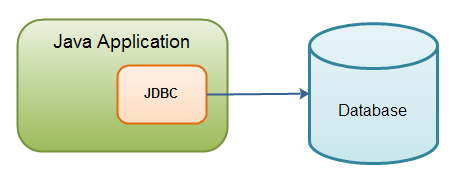
\includegraphics[scale=0.7]{../graph/jdbc.png} \\
  \caption{Schéma simple du JDBC - http://tutorials.jenkov.com/jdbc/index.html}
\end{figure}

L'API JDBC est composée des interfaces et classes suivantes :
\begin{description}
 \item[Driver :] cette interface gère les communications avec le serveur de base de données. On ne l'utilise pas directement, on utilisera plutôt le DriverManager.
 \item[DriverManager :] cette classe gère la liste des pilotes de base de données. Il choisira à la connexion le pilote correspondant à la base utilisée.
 \item[Connection :] cette interface contient toutes les méthodes permettant d'échanger avec la base de données.
 \item[Statement :] cette interface permet de soumettre des requêtes SQL à la base de données.
 \item[ResultSet :] cette classe contient les données récupérées suite à une requête à la base de données après son exécution.
 \item[SQLException :] cette classe gère les différentes erreurs qui peuvent se produire lors de l'accès à la base de données. 
\end{description}

\subsubsection{Mise en place}

Une fois que le pilote est chargé dans le code Java, on se connecte à la base de données voulue avec l'URL, l'utilisateur et le mot-de-passe. Le package java.sql est ici nécessaire. Lorsque la connexion a été établie, l'exécution d'une requête se fait de la manière suivante :
\begin{lstlisting}
  // Chargement du pilote :
  Class.forName("com.mysql.jdbc.Driver").newInstance();
  
  // Connexion a la base de donnees :
  java.sql.Connection connexion =  DriverManager.getConnection("jdbc:mysql:URL", "utilisateur", "motDePasse");
  
  // Generation de l'objet statement associe à la connexion :
  java.sql.Statement statement = connexion.createStatement();
\end{lstlisting}  
  
Maintenant que la connexion est établie, il est possible d'interagir avec la base de données. Dans les exemples ci-dessous, nous supposerons que la base de données est composée d'une table Joueur dont les attributs sont des chaînes de caractères représentant le nom et le prénom des joueurs. Il existe deux fonctions principales associées à différents types de requêtes et qui s'appliquent à l'objet Statement :
\begin{itemize}
 \item \textit{executeQuery(String sql)} : permet d'exécuter une requête du type 'SELECT' par exemple et qui donne retourne certaines lignes d'une table.
\begin{lstlisting}  
  // Ecriture et execution de la requete SQL :
  String requete = "SELECT * FROM Joueur";
  ResultSet resultat = statement.executeQuery(requete);
\end{lstlisting}
 \item \textit{executeUpdate(String sql)} : permet de mettre à jour une table de la base de données dans le cadre de requêtes du type 'UPDATE', 'INSERT', 'DELETE'.
\begin{lstlisting}
  // Mise a jour d'une table (ajout d'un joueur) :
  String udpate = "INSERT INTO Joueur (nom, prenom) VALUES ('Dupont', 'Jean')";
  int nbLignesMAJ = statement.executeUpdate(update);
\end{lstlisting}
\end{itemize}

Une fois que la requête a été exécutée, il ne reste plus qu'à lire les données reçues. Dans le cadre de l'utilisation de la fonction executeUpdate, on récupère simplement un entier qui donne le nombre de lignes mise à jour dans la table. En revanche, la fonction executeQuery retourne un objet du type ResultSet qui est moins trivial à étudier. Cet objet contient une certain nombre de lignes répondant aux conditions de la requête et peut être comparé à une table d'une base de données. Il est composé de colonnes symbolisant les attributs des enregistrements de la table : ils possèdent un nom et un domaine dans lequel ils prennent leur valeur (int, float, char, ...). De plus, pour parcourir cet objet on a une sorte de curseurs qui point sur une ligne. On utilise la commande next pour passer à la ligne suivante si elle existe.
\begin{lstlisting}  
  // Parcours du ResultSet s'il est non nul et tant qu'il y a une ligne :
  Vector<String> noms;
  Vector<String> prenoms;
  if (resultat != null) {
    while (resultat.next()) {
      noms.add(resultat.getString("nom"));
      prenoms.add(resultat.getString("prenom"));
    }
  }
\end{lstlisting}

Après l'exécution de requêtes et la récupération des données, il ne reste plus qu'à 'refermer' la connexion de la manière suivante :
\begin{lstlisting}
  // Fermeture des ojets :
  statement.close();
  connexion.close();
\end{lstlisting}

Les exemples de codes précédents ne prennent pas en compte les erreurs pouvant être générées lors de la compilation de ce code. En réalité, il faut protéger les instructions et lever les exceptions générées. Voici les erreurs qui peuvent être générées :
\begin{itemize}
 \item Lors de la connexion : échec de la connexion (ex : mauvais mot de passe, URL invalide,...).
 \item Lors de l'exécution d'une requête : mauvaise syntaxe ou appel de table/attributs inexistants.
 \item Lors de la déconnexion.
\end{itemize}

\subsubsection{Avantage et Inconvénient}
Il existe d'autre moyens d'accéder à une base de données MySQL en Java tel que Hibernate mais il s'utilise dans le cadre d'une architecture ORM (Objet/Relational Mapping) alors que nous allons utliser une architecture DAO (Data Access Object) pour l'accès à notre base de données. L'avantage du JDBC est qu'il est simple à utiliser (seulement deux méthodes pour exécuter des requêtes SQL) et qu'il contient des pilotes permettant d'accéder à n'importe quelle base de données de type relationnel.


%%%%%%%%%%%%%%%%%%%%%%%%%%%%%%%%%%%%%%%%%%%%%%%%%%%%%%%%%%
%----------------------DAO-------------------------------%
%%%%%%%%%%%%%%%%%%%%%%%%%%%%%%%%%%%%%%%%%%%%%%%%%%%%%%%%%%
\subsection{DAO}

\subsubsection{Présentation}
Un objet d'accès aux données (Data Access Object ou DAO en anglais) est un modèle qui permet d'isoler les méthodes concernant le stockage des données et de ne pas les écrire directement dans nos classes métier. Ainsi le modèle DAO permet de regrouper l'accès aux données dans des classes à part plutôt que de les disperser. \\

Le but du modèle DAO est d'arriver à encapsuler les méthodes concernant la communication avec la base de données dans une couche pour arriver au schéma suivant :

\begin{figure}[!h]
  \center
  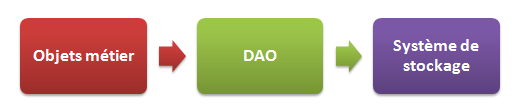
\includegraphics[scale=0.5]{../graph/dao1.png} \\
  \caption{Schéma simple du modèle DAO}
\end{figure}

\subsubsection{Mise en place}
La couche DAO va gérer les opérations classiques de stockage : ajout, lecture, modification et suppression. Ces quatre opérations sont souvent raccourcis par l'acronyme CRUD (create, read, update and delete). \\

Pour mettre en application le modèle DAO nous avons du créer nos propres exceptions. En effet, il faut que les exceptions générées par SQL ou JDBC soit référencées comme étant des exceptions dues à la boite noire DAO. 

En reprenant la même idée, DAO se propose d'offrir une interface pour chacun des objets décrivant l'ensemble des méthodes qui seront accessibles dans l'objet. Ainsi, peu importe l'implémentation effectuée on pourra connaître les diverses méthodes de nos classes. Les interfaces permettent de décrire les méthodes des objets la couche donnée et ce n'est que l'implémentation qui sera dépendante du mode de stockage. Par exemple, pour un stockage SQL nous pouvons utiliser le driver JDBC présenté ci-dessus.\\ 
\begin{figure}[!h]
  \center
  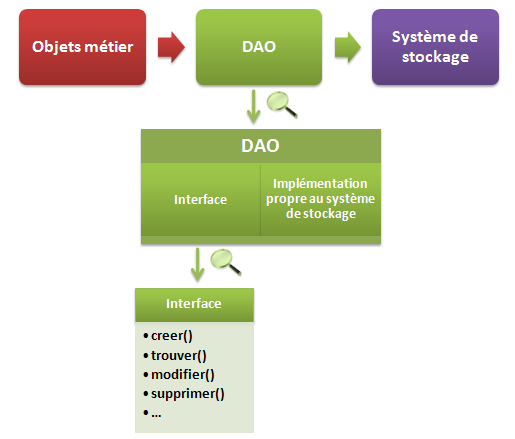
\includegraphics[scale=0.5]{../graph/dao2.png} \\
  \caption{Schéma détaillé du modèle DAO}
\end{figure}

La couche DAO comportera également une fabrique. Cette fabrique sera unique et ne sera instanciée que si les informations de configuration sont correctes. Le but de cette fabrique sera de fournir une instance des différentes implémentations de la DAO.

\subsubsection{Avantage et Inconvénient}
L'avantage du modèle DAO est donc clair, le changement du mode de stockage de données est simple. En effet, nous aurons seulement à changer nos classes DAO pour changer ce mode de stockage. L'inconvénient est du à la mise en œuvre qui demande une couche supplémentaire. 



%%%%%%%%%%%%%%%%%%%%%%%%%%%%%%%%%%%%%%%%%%%%%%%%%%%%%%%%%%
%----------------------Serialisation---------------------%
%%%%%%%%%%%%%%%%%%%%%%%%%%%%%%%%%%%%%%%%%%%%%%%%%%%%%%%%%%
\subsection{La sérialisation}

\subsubsection{Principe}

La sérialisation est le processus de conversion d'un objet pour l'enregistrer dans une base de données ou un fichier par exemple. Le processus inverse s'appelle la désérialisation. Nous pouvons donc représenter cette méthode selon le schéma suivant. 

\begin{figure}[!h]
  \center
  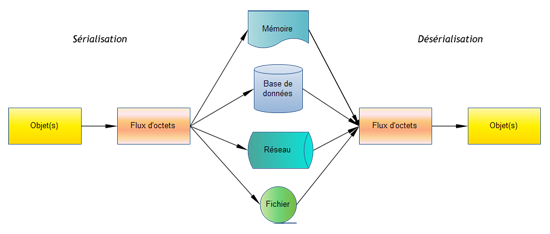
\includegraphics[scale=0.5]{../graph/serialisation.png} \\
  \caption{Schéma de la sérialisation}
\end{figure}

\subsubsection{Mise en place}
On peut choisir par exemple d'effectuer sa sérialisation en XML. \\

La classe XMLEncoder permet de sérialiser un objet en XML. Cette sérialisation ne prend en compte que les champs ayant un getter et un setter public. XMLEncoder(output) crée une nouvelle instance qui utilise le flux passé en paramètre comme résultat de la sérialisation. \\

La classe XMLDecoder permet quand à elle de désérialiser un objet à partir d'un document XML. \\

Pour notre application nous aurions besoin d'effectuer une sérialisation vers SQL. Prenons l'exemple du joueur, pour effectuer la sérialisation nous avons besoin d'une classe Joueur qui implémente Serializable, d'avoir un constructeur par défaut et d'avoir un getter et un setter public pour chaque attribut. Ensuite notre table SQL java doit contenir un id et un longblob (Binary Large Object). Ensuite nous n'avons plus qu'a effectue une sauvegarde dans la base de données. Pour la desérialisation, il nous faut récupérer le longblob pour le convertir en ObjectInputStream pour utiliser la méthode readObject(). 


\subsubsection{Avantage et Inconvénient}
La sérialisation présente des avantages comme une bonne portabilité ou le fait que le processus de sérialisation ne prenne pas en compte les champs qui ont leur valeur par défaut. Elle présente les inconvénients suivants : 
\begin{itemize}
\item ne peut s'utiliser que sur des objets respectant la convention JavaBeans (constructeur par défaut, getter et setter pour tous les attributs ..)
\item la taille des données sérialisés est plus importante que leur équivalent binaire
\end{itemize}


%%%%%%%%%%%%%%%%%%%%%%%%%%%%%%%%%%%%%%%%%%%%%%%%%%%%%%%%%%
%----------------------CHOIX-----------------------------%
%%%%%%%%%%%%%%%%%%%%%%%%%%%%%%%%%%%%%%%%%%%%%%%%%%%%%%%%%%
\subsection{Notre choix : DAO vs Serialisation}
Pour la communication avec notre base de données nous avons choisi d'utiliser le modèle DAO. \\

Le modèle DAO demande plus de travail pour être mis en place que la sérialisation mais possède l'avantage de nous fournir une base de données plus facilement utilisable dans un autre contexte. En effet, chacune de nos tables ne seront pas simplement un blob mais une valeur pour chacun des champs de notre table. 
	
	\section{Cryptage du mot de passe}

Lors du déroulement du jeu nous allons avoir besoin de stocker le mot de passe du joueur. Pour cela, nous avons pensé qu'il était préférable d'encrypter ce mot de passe lors de son stockage. \\
Nous avons ainsi chercher différentes méthodes pour effectuer l'encryptage du mot de passe. 

\subsection{Fonctions SQL}

Dans le langage SQL, la fonction MDA5() permet de chiffrer une chaîne de caractère en un entier hexadécimal de 32 caractères. \\
L'algorithme MDA() est une fonction de hachage cryptographique qui calcule à partir d'une chaîne de caractère son empreinte avec une probabilité très forte que deux empreintes soient différentes. Depuis 2004, une équipe chinoise a découvert des collisions complètes et MD5 n'est donc plus considéré comme sur au sens cryptographique. \\

La fonction SQL SHA1() permet de chiffrer une chaîne de caractère sous la forme d'un chaîne de caractères de 40 caractères. SHA1 est également une fonction de hachage cryptographique. Elle a l'avantage d'être considéré comme sur contrairement à MDA(). 



\subsection{Jasypt}
Jasypt est une librairie java qui permet d'encrypter facilement les mots de passe avec une une grande sécurité. \\
Jasypt possede les avantages suivants :
\begin{itemize}
\item il permet de choisir la fonction de hachage que nous souhaitons (MDA ou SHA par exemple)
\item il ajoute un salage au mot de passe qui permet d'avoir deux mots de passe cryptés différents pour le même mot de passe de départ
\item il applique un nombre aléatoire de fois notre fonction de hachage (nombre > 1000 pour rendre plus difficile les attaques)
\end{itemize}  

Le code pour encrypter le mot de passe est très simple, il nous suffit de créer un objet de type ConfigurablePasswordEncryptor, de définir l'algorithme de chiffrement. La méthode setPlainDigest nous permet avec l'argument false de choisir la méthode la plus sure avec un salage et un nombre d'itération aléatoire pour notre fonction de hachage. Enfin il ne nous reste plus qu'a appeler la méthode encryptPassword qui nous renvoie notre mot de passe encrypté à partir d'un mot de passe donné en entrée. 
\begin{lstlisting}
 ConfigurablePasswordEncryptor passwordEncryptor = new ConfigurablePasswordEncryptor();
 passwordEncryptor.setAlgorithm( ALGO_CHIFFREMENT );
 passwordEncryptor.setPlainDigest( false );
 String motDePasseChiffre = passwordEncryptor.encryptPassword( motDePasse );
\end{lstlisting} 


De même que pour vérifier que notre mot de passe correspond au mot de passe chiffré il existe une méthode qui nous renvoie vraie en cas de correspondance :

\begin{lstlisting}
passwordEncryptor.checkPassword(motDePasse, motDePasseChiffre )
\end{lstlisting}


\subsection{Notre choix}
L'inconvénient d'utiliser les fonctions de SQL est que l'on choisi une manière de crypter dépendante de notre base de données. Si nous décidons de changer notre manière de stocker notre base de données nous devrons ainsi trouver une nouvelle fonction. \\

Nous avons donc choisi d'utiliser Jasypt pour encrypter notre mot de passe. Cette librairie a l'avantage de nous permettre d'encrypter uen chaîne de caractère de manière relativement sure sans avoir de grandes compétences en cryptographie. En effet, nous ne connaissons pas en détail le fonctionnement de l'algorithme de cryptage mais avons simplement une idée globale de son fonctionnement. \\

Nous avons choisi comme fonction de hachage (ALGOCHIFFREMENT) SHA car nous avons que MDA n'est plus sur. Une fois l'encryptage du mot de passe effectué nous obtenons une chaîne de caractères de taille 56.
	
	\section{Gestion des cours de la bourse : Yahoo! Finance}

Dans le cadre de ce projet nous avons besoin de connaître les cours des indices et des actions pour pouvoir permettre au joueur de faire des paris sur ce qu'il va se passer.

\subsection{Présentation}

Yahoo! Finance est un site internet du groupe Yahoo! qui délivre des nombreuses informations dans le domaine de la finance. Ainsi, nous retrouvons une section actualité qui nous permet d'avoir un rapide coup d’œil sur les divers articles de journaux en rapport avec l'économie. Dans la partie vidéo le principe est le même sauf que les actualités sont sous forme de vidéos. \\

Yahoo propose de visualiser de nombreuses informations en rapport avec les cours ou indices. \\

Par exemple, pour l'indice du cac 40 n retrouve sa valeur ainsi que va variation par rapport à la dernière session. On a accès à la dernière valeur de clôture ainsi que la valeur à l'ouverture. Un graphique représente l'évolution du prix de l'indice depuis l'ouverture de la session. Nous avons également accès aux articles concernant le CAC40 dans la presse écrite, aux composants du CAC40 ainsi qu'aux prix historiques (valeur ouverture, fermeture, haut, bas sur la période désirée). \\


Pour un indice, ACCOR S.A dans notre exemple la page se présente comme suit : \\
\begin{figure}[H]
  \center
  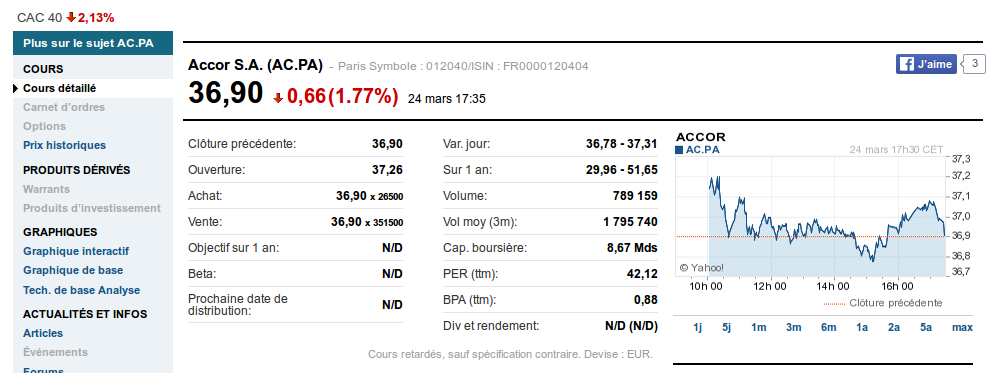
\includegraphics[scale=0.4]{../graph/yahoo.png} \\
  \caption{Visualisation du site Yahoo! Finance}
\end{figure}
Nous retrouvons les prix historiques (ce qui nous intéresse) ainsi que d'autres informations concernant le cours. 

\subsection{Principe du téléchargement}

Nous avons vu dans la partie précédente que nous avions accès à l'historique des cours pour les indices et les cours. Nous avons la possibilité de télécharger ces cours au format CSV. La chose intéressante à étudier est la construction de l'URL qui permet d'effectuer ce téléchargement. \\ 

Par exemple, regardons l'URL pour télécharger le cours d'IBM entre le 01 janvier 2016 et le 01 février : 
\begin{lstlisting}
real-chart.finance.yahoo.com/table.csv?s=IBM&a=00&b=1&c=2016&d=01&e=1&f=2016&g=d&ignore=.csv
\end{lstlisting}
Nous pouvons ainsi étudié la construction de l'URL qui sera la même pour télécharger chacun des cours. L'URL est construit de la manière suivante : 
\begin{itemize} 
\item "real-chart.finance.yahoo.com/table.csv?" une première partie fixe qui sera commune à tous les téléchargements 
\item "s=IBM" qui permet de savoir quel action/indice nous téléchargeons. Ici IBM correspond au code d'IBM sur la site Yahoo! Finance
\item "\&a=00\&b=1\&c=2016" correspond à la date à partir de laquelle nous souhaitons télécharger les valeurs, "a" correspond au mois (00 = janvier), b au jour, et c à l'année
\item "\&d=01\&e=1\&f=2016" correspond à la date jusqu'à laquelle nous souhaitons télécharger les valeurs, "d" correspond au mois (01 = février), e au jour, et f à l'année
\item "\&g=d" signifie que nous voulons télécharger les valeurs jour par jour, nous aurions pu choisir semaine par semaine ou mensuellement
\item "\&ignore=.csv" enfin cela signifie que nous voulons télécharger au format csv
\end{itemize}

Une fois cette remarque effectuée nous voyons que le code pour télécharger le cours est très simple : 

\begin{lstlisting}
//Construisons l'url de notre page
		//Chaque url permettant d'acceder aux cours de la bourse est construit de la meme maniere
String url="http://real-chart.finance.yahoo.com/table.csv?"+
		           "s="+code  //code correspondant a l'action
		           +"&a="+debut.get(Calendar.MONTH) //mois de debut 00=janvier, 01=fevrier, 02=mars...
		           +"&b="+debut.get(Calendar.DAY_OF_MONTH) //jour de debut
		           +"&c="+debut.get(Calendar.YEAR) //annee de debut
		           +"&d="+fin.get(Calendar.MONTH)
		           +"&e="+fin.get(Calendar.DAY_OF_MONTH)
		           +"&f="+fin.get(Calendar.YEAR)
		           +"&g=d" //On veut par jour
		           +"&ignore=.csv"; //au format csv;
		
		//Il ne nous reste plus qu'a nous connecter a l'url et copier les donnees
		try
		{
			URL yahooUrl = new URL(url);
			URLConnection donnee = yahooUrl.openConnection();
			Scanner entree = new Scanner(donnee.getInputStream());
			
			while(entree.hasNextLine()){
				String ligne = entree.nextLine();
				Traitement de la ligne
			}	
		}
		catch(Exception e)
		{
			System.err.println(e);
		}
\end{lstlisting} 
	
	\section{Affichage et visualisation des cours}

L'un des objectifs de notre projet étant de fournir à l'utilisateur une IHM pour visualiser les cours ainsi que des indicateurs financiers via l'analyse technique que nous verrons dans le chapitre suivant, nous avons besoin d'afficher des graphes et autres diagrammes.
Par exemple, nous pourrions vouloir afficher l'historique d'un cours sur une période ou encore visualiser la répartition des actifs d'un portefeuille sous forme diagramme en camembert. Le graphique doit donc être afficher sur une page web sachant que nous utilisons une plateforme Java EE.\\

Pour cela, plusieurs possibilités s'offraient à nous :
\begin{itemize}
 \item Publier les graphiques en 'Flash',
 \item Générer des graphes sous forme d'image puis les afficher,
 \item Utiliser une générateur Javascript permettant l'affichage de graphiques.
\end{itemize}

Nous allons présenter un exemple de chacune de ces possibilités que nous aurions pu utiliser puis nous expliquerons notre choix.

%-------------------------------------------------------------------%
%------------------------FusionCharts-------------------------------%
%-------------------------------------------------------------------%
\subsection{Graphiques en Flash : FusionCharts Free}

\subsubsection{Présentation de Flash}
Flash est une technologie qui permet de manipuler des graphiques vectoriels, des bitmaps et certains scripts utilisés dans les applications web, les jeux et les vidéos. L'avantage de Flash est qu'il est répandu sur de nomreux logiciels et nombreux systèmes d'exploitation.\\

Les fichiers Flash ont pour extension '.swf' et peuvent être inclus dans une page web puis lus par le plugin Flash du navigateur. Sinon, ils peuvent être interprétés de manière indépendante dans le lecteur Flash Player.\\
Aujourd'hui, le plugin Flash est la technologie la plus utilisée dans les navigateurs web pour afficher du contenu multimédia. On se pose néanmoins la question de son remplacement par HTML5 dans un futur proche.\\
Le lecteur Flash permettant la lecture des fichiers multimédias a été développé par Adobe Systems et est compatible avec la plupart des systèmes d'exploitation et navigateurs.
\begin{figure}[H]
  \center
  
\includegraphics[scale=0.4]{../graph/flashAdobe.jpg}
  \caption{Adobe Flash Player - \url{http://www.adobe.com/fr/products/flashplayer.html}}
\end{figure}
D'autres projets de lecteurs Flash existent mais ne sont pas aboutis.

\subsubsection{FusionCharts Free}
FusionCharts Free est un composant open-source permettant d'intégrer des graphes intéractifs et animés dans une application web. Il utilise la technologie Flash décrite précédemment. Il existe une version gratuite 'FusionCharts Free', c'est un logiciel multiplate-forme qui peut être implémenté avec toute sorte de technologies comme PHP, .NET, Python, JSP ou même un simple HTML.\\

On s'intéresse à la version qui utilise les JSP car c'est celle que l'on pourrait utiliser dans notre projet.
On peut trouver les guides et téléchargements nécessaires sur le site Internet :
\begin{figure}[H]
  \center
  
\includegraphics[scale=0.8]{../graph/fusionCharts.png}
  \caption{FusionCharts Free - \url{http://www.fusioncharts.com/goodies/fusioncharts-free/}}
\end{figure}

Les étapes pour la mise en place d'un graphe sur une page web sont les suivantes :
\begin{enumerate}
 \item \textbf{Mettre en place les données :} possibilité de fournir les données sous forme JSON ou XML. Cela peut être une chaîne de caractères ou un fichier. Voici un exemple en XML que nous pourrions utiliser et qui serait placé dans un fichier Donnees.xml :
\begin{lstlisting}[language=XML]
<graph caption="Revenus trimestriels 2015" xaxisname="Trimestres" yaxisname="Revenus (euros)">
    <set label="T1" value="420000" />
    <set label="T2" value="810000" />
    <set label="T3" value="720000" />
</graph>
\end{lstlisting}
 \item \textbf{Inclure le code HTML pour intégrer l'objet Flash et fournir les paramètres nécessaires :} cette étape est fourni par le développeur dans un fichier JSP téléchargeable sur le site (FusionChartsHTMLRenderer.jsp). Il suffira alors d'inclure le fichier dans la page web où l'on souhaite afficher un graphe. Il ne reste plus donc qu'à intégrer le code suivant dans les balises HTML de notre JSP.\\
 Le paramètre chartSWF précise la forme de graphe utilisée (ici un colonne en 3D), on place nos données dans strURL ou strXML suivant si on utilise l'URL d'un fichier ou si on défini dans une variable locale les données.
 Chaque graphe d'une page doit avoir un ID unique, que l'on choisit dans le paramètre chartId. On peut également choisir la hauteur et la largeur du graphe qui s'affichera.
\begin{lstlisting}[language=HTML]
<jsp:include page="../Includes/FusionChartsHTMLRenderer.jsp" flush="true">
    <jsp:param name="chartSWF" value="../../FusionCharts/FCF_Column3D.swf" />
    <jsp:param name="strURL" value="Data/Donnes.xml" />
    <jsp:param name="strXML" value="" />
    <jsp:param name="chartId" value="graphe1" />
    <jsp:param name="chartWidth" value="600" />
    <jsp:param name="chartHeight" value="300" />
</jsp:include>
\end{lstlisting} 
 \item \textbf{Visualiser le graphe sur la page web :} avec les exemples précédents et des données un peu plus détaillées, on obtiendrait un graphe comme le suivant.
\begin{figure}[H]
  \center
  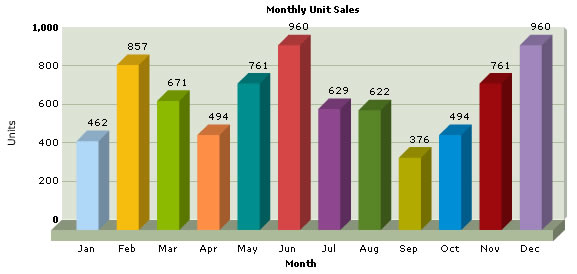
\includegraphics[scale=0.6]{../graph/fusionChartsExemple.jpg}
  \caption{Exemple de graphe en colonne 3D avec FusionCharts Free - \url{http://docs.fusioncharts.com/free/}}
\end{figure}
\end{enumerate}


%-------------------------------------------------------------------%
%------------------------JFreeChart---------------------------------%
%-------------------------------------------------------------------%
\subsection{Images de graphes : JFreeChart}
\subsubsection{Présentation}
JFreeChart est une API Java qui permet de créer des graphes et diagrammes en Java. Elle est open source mais la documentation est payante. Elle se présente sous la forme d'une librairie qui peut être intégrée à l'IDE Eclipse.
\begin{figure}[H]
  \center
  
\includegraphics[scale=0.5]{../graph/JFreeChart.png}
  \caption{JFreeChart - \url{http://www.jfree.org/jfreechart/}}
\end{figure}

JFreeChart permet de tracer différents graphes et ce avec une très bonne qualité d'image. On peut par exemple citer les diagrammes en bar (bar charts), les camemberts (pie charts), les histogrammes, parmis bien d'autres.

Pour utiliser cette librairie, il suffit de la télécharger sur le site suivant : \url{https://sourceforge.net/projects/jfreechart/files/}.
Il faut ensuite extraire l'archive et intégrer le .jar au projet dans Eclipse.

\subsubsection{Mise en place}
Nous allons aborder l'utilisation de JFreeChart avec des JSP. Le principe est que nous allons créer le graphe puis l'enregistrer sous forme d'image. Nous afficherons ensuite l'image dans la page web que l'on souhaite.\\

Il faut donc :
\begin{enumerate}
 \item Créer le graphe dans une JSP et le sauvegarder en variable de session par exemple.
 \item Créer l'image 'map' à partir de ce graphe.
 \item Récupérer l'image dans la servlet et l'enregistrer sous forme de fichier.
 \item Afficher l'image dans la JSP correspondant à la page web dans laquelle on souhaite visualiser le graphe.
\end{enumerate}

Une simplification est d'utiliser Cewolf qui est basé sur JFreeChart et peut être utilisé dans une application web basée sur les JSP et les servlets. En utilisant Cewolf, on n'a plus besoin de stocker l'image car tout se fait de manière dynamique.\\
\begin{figure}[H]
  \center
  
\includegraphics[scale=0.5]{../graph/Cewolf.png}
  \caption{Cewolf - \url{http://cewolf.sourceforge.net/new/index.html}}
\end{figure}

Cewolf est bien documenté est on peut réaliser notre graphique en suivant les étapes suivantes :
\begin{enumerate}
 \item \textbf{Préparer l'application :} ajouter les librairies (.jar) dans le dossier /WEB-INF/lib du projet disponible sur la page \url{https://sourceforge.net/projects/cewolf/files/}.
 \item \textbf{Préparer les données :} créer un objet qui implémente l'interface DatasetProducer (propre à Cewolf). Cela revient à créer une classe qui implémente cette interface. Elle devra implémenter les méthodes \textit{produceDataset()} (pour les données du graphe), \textit{hasExpired} (pour savoir si les données ne sont plus à jour) et \textit{getProducerId()} (identifie le type de DatasetProducer, si deux ont le même ID, ils produisent les même données).
 \item \textbf{Ajouter la servlet Cewolf à l'application :} la classe servlet est déjà fournie avec Cewolf, il suffit de l'ajouter au fichier de configuration web.xml.
 \item \textbf{Définir le graphe dans la JSP :} à l'aide des balises (tags) \textit{<cewolf:chart>}, \textit{<cewolf:data>} et \textit{<cewolf:img>} on intègre l'image à la page JSP dans le bloc HTML. On peut y préciser le titre du graphe, les axes, les dimensions, etc...
\end{enumerate}

La mise en place est assez complexe, mais au final on peut obtenir des graphes sous forme d'image comme les suivants :
\begin{figure}[H]
  \center
  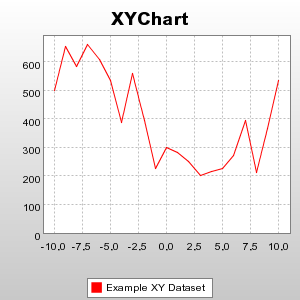
\includegraphics[scale=0.5]{../graph/cewolfEx1.png}
  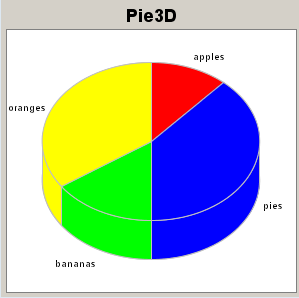
\includegraphics[scale=0.5]{../graph/cewolfEx2.png} 
  \caption{Exemples avec Cewolf - \url{http://cewolf.sourceforge.net/new/index.html}}
\end{figure}

%-------------------------------------------------------------------%
%------------------------GoogleChart--------------------------------%
%-------------------------------------------------------------------%
\subsection{Javascript : API Google Chart}
\subsubsection{Présentation}
L'API Google Chart est un outil qui permet de créer facilement des graphes à partir de données et de l'afficher dans une page web. Les graphes sont intéractifs et peuvent être personnalisé. Il existe de nombreux types de graphes disponibles allant du graphe linéaire à l'histogramme en passant par des organigrammes ou encore des cartes géographiques.\\
\begin{figure}[H]
  \center
  
\includegraphics[scale=0.5]{../graph/googleAPI.png}
  \caption{API Google Chart - \url{https://developers.google.com/chart/}}
\end{figure}

Cette API se met en place en Javascript sans que l'on est besoin de télécharger quoi que ce soit. Il suffit d'avoir une connexion Internet pour afficher les graphes.

\subsubsection{Mise en place}
Pour utiliser les graphes mis à disposition par Google, il faut suivre le schéma suivant et écrire le code dans les balises HTML de la page JSP dans laquelle on souhaite afficher un graphe :
\begin{enumerate}
 \item \textbf{Charger la librairie :} nous n'aurons besoin que de graphes classiques, c'est pourquoi on charge uniquement le package intitulé 'corechart'. Le mot clé 'current' signifie que l'on veut charger la dernière mise à jour officielle et validée par Google Charts. De plus, on suppose que l'on aura une fonction JavaScript plus loin dans le code intitulée 'drawChart'.
\begin{lstlisting}
<script type="text/javascript" src="https://www.gstatic.com/charts/loader.js"></script>
<script type="text/javascript">
    google.charts.load('current', {packages: ['corechart']});
    google.charts.setOnLoadCallback(drawChart);
</script>
\end{lstlisting}
 \item \textbf{Préparer les données :} l'API requiert d'avoir les données sous forme d'une 'DataTable' qui est une classe Javascript définie dans la librairie Google Visualization chargée à l'étape précédente. Une DataTable est un tableau à deux dimensions donc les colonnes sont les types de données et les lignes les données elle-mêmes. Il existe différentes manières de créer une DataTable mais il est important qu'elle soit toujours adaptée au type de graphe qui sera créé (par exemple pour un camembert il faudra toujours deux colonnes). Il est possible d'instancier la DataTable de manière statique ou dynamique. Remarque : tous les morceaux de code qui suivent devront être placés dans une fonction Javascript \textit{drawChart} comme précisé précédemment.
\begin{lstlisting}
// Creation de la DataTable avec deux colonnes et trois lignes :
var data = new google.visualization.DataTable();
data.addColumn('string', 'Actifs');
data.addColumn('number', 'Quantite');
data.addRows([
    ['Obligation', 76.7],
    ['Action', 23.3]
]);
\end{lstlisting}
 \item \textbf{Personnaliser le graphe :} il est possible de spécifier certaines options à l'API comme les couleurs de chaque partie du graphique, la police, la taille, le titre, les légendes, etc...
\begin{lstlisting} 
var options = {
    backgroundColor: '#d2d2d2',
    title: 'Repartition du portefeuille selon la somme investie',
    is3D: true,
    width:400,
    height:300
};
\end{lstlisting}
 \item \textbf{Dessiner le graphe :} c'est ici que l'on va préciser à l'API quel type de graphe on souhaite dessiner, avec quelles données et options. On affectera alors un ID au graphique qui servira dans la dernière étape. Remarque : après ces deux lignes, la fonction \textit{drawChart} est finie.
\begin{lstlisting}
var chart = new google.visualization.PieChart(document.getElementById('camembert'));
chart.draw(data, options);
\end{lstlisting} 
 \item \textbf{Afficher le graphe :} il ne reste plus qu'à choisir l'emplacement du graphe dans la page web et à insérer la ligne suivante au bon endroit dans le HTML. L'ID devra être exactement le même que celui donné dans l'étape précédente.
\begin{lstlisting}
<div id="camembert"></div>
\end{lstlisting}  
 
 On est censé voir s'afficher ceci :
\begin{figure}[H]
  \center
  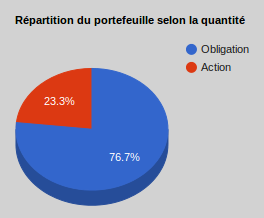
\includegraphics[scale=0.6]{../graph/camembertAPI.png}
  \caption{Exemple diagramme Camembert (Pie Chart)}
\end{figure}
\end{enumerate}


%-------------------------------------------------------------------%
%------------------------notrechoix---------------------------------%
%-------------------------------------------------------------------%
\subsection{Notre choix}
Maintenant que nous avons étudié les différentes options qui s'offrent à nous, nous pouvons discuter la meilleure solution à adopter. Tout d'abord, il apparait clairement que la méthode utilisant Flash est désuette bien qu'elle doit fonctionner sans problème. Nous n'avons donc même pas essayé de l'implémenter.\\

En ce qui concerne la librairie JFreeChart, c'est la première à laquelle nous avons pensé et que nous avons essayé de mettre en oeuvre. Après avoir rencontré quelques difficultés dans la mise en place de cette solution, nous avons réfléchis à une autre solution. En effet, nous perdions trop de temps à essayer d'utiliser JFreeChart et Cewolf, sans parler du fait que cela nécessitait l'ajout de librairie à notre projet.\\

Ainsi, nous nous sommes finalement retrouvé à utiliser l'API Google Chart qui, pour le coup, est très simple à utiliser car elle est gérée uniquement dans les JSP. De plus, nous trouvons que les graphes mis à disposition sont satisfaisants et que l'intéractivité avec les diagrammes peut avoir des avantages lors de l'analyse des graphes.\\

Nous avons néanmoins rencontré quelques difficultés avec les DataTable lorsque nous avons voulu les définir de manière dynamique, mais nous avons finalement réussi et ce notamment grâce à la librairie JSTL que nous avons défini auparavant.
	
	
\chapter{Théorie Finance}
	\section{Définitions}

\subsection{Les marchés}

Lorsqu'un acheteur et un vendeur souhaitent conclure une transaction, ils peuvent le faire sur deux types de marché : le marché organisé ou le marché gré à gré.  

\subsubsection{Marché organisé}
Dans un marché organisé, l'acheteur et le vendeur placent des ordres d'achats et de vente via une société de bourse telle que NYSE Euronext par exemple. \\

Une société de bourse est une société commerciale ayant pour but d'organiser le marché financier en fixant des règles de fonctionnement et d'admission au marché. Ces règles doivent respecter celles définies par l'autorité des marchés financiers (AMF) en France. Le marché organisé n'est donc pas ouvert à tous, les membres de ce marché peuvent ainsi transmettre les ordres de leurs clients, qu'ils soient particuliers ou institutionnels. Un membre de ce marché peut être par exemple un courtier. \\

Sur un marché organisé il existe une chambre de compensation qui a pour objectif de garantir la finalité des opérations aux vendeurs et acheteurs. Pour pouvoir participer au marché organisé il faut payer des frais de gestion. 

\subsubsection{Marché gré à gré}
Dans un marché gré à gré, la transaction est conclue bilatéralement entre les deux parties. \\

Dans ce marché, les règles sont donc plus souples car il est possible de discuter directement avec l'acheteur (respectivement le vendeur) pour définir toutes les clauses du contrat comme un paiement échelonné par exemple.  

\subsubsection{Marché primaire}
C'est un lieu où sont émis les nouveaux titres.

\subsubsection{Marché primaire}
C'est le lieu ou l'acheteur peut revendre ses titres à un cours défini par la rencontre de l'offre et la demande. 

\subsection{Les différents produits financiers}

\subsubsection{Action}
Une action représente une part du \textbf{capital} de la société émettrice. Dés qu'une société est cotée en bourse, les actions qui composent son capital social vont évoluer en fonction des achats et des ventes des investisseurs en suivant le jeu de l'offre et de la demande.  \\
En achetant une action, on fait grimper le prix. Au bout d’un moment, le prix du marché de l’action va dépasser sa fair value, on décide alors de la vendre pour cristalliser le bénéfice gagné. En vendant une action, on fait alors baisser le prix.\\ 

Le détenteur d'actions est qualifié d'actionnaire et l'ensemble des actionnaires constitue l'actionnariat. \\


Les action donnent des droits à leurs propriétaires : 
\begin{itemize}
\item Droits politiques : droit à l'information et au vote
\item Droits financiers : droit aux dividendes
\end{itemize}

\subsubsection{Indice boursier}
Un indice boursier est un panier d'actions dont les variations sont supposées refléter au mieux les fluctuations d'un marché (par exemple le marché français) ou d'un secteur d'activité particulier (par exemple l'indice sectoriel du secteur aéronautique). \\

Un indice boursier est un outil statistique qui est calculé à partir de la moyenne des titres qui le composent. En général, cette moyenne est pondéré : certains actifs ont un poids plus fort. Cette pondération peut-être fonction de la capitalisation boursière par exemple (nombre d'actions émises multipliées par leurs valeurs. Euronext (principal opérateur financier de la zone euro) permet de prendre connaissance et de suivre tous les indices boursiers de la zone euro.  \\

Les principaux indices boursiers du marché français sont les suivants :
\begin{itemize}
\item Le CAC40 (Cotation Assistée en Continu est l'indice de référence de la place de Paris. Il a été créé en 1998 avec une base de 1000 points et est constitué des quarante plus grandes valeurs cotées en continu à la bourse de Paris. 
\item Le SBF 120 (Société des Bourses Françaises) est composé des 40 valeurs du CAC40, des 20 valeurs de l'antichambre du CAC40 (CAC Next 20) et des 60 valeurs les plus liquides de la bourse de Paris.
\item CAC All-Tradable a remplacé le SBF 250 en 2011 et représente les 250 valeurs les plus importantes de la bourse de Paris.  
\end{itemize}

Les principaux indices boursiers mondiaux : 
\begin{itemize}
\item Le Dow Jones est le plus vieil indice boursier du monde, il est l'indice le plus important de New-York. Il est composé des 30 valeurs américaines les plus importantes. 
\item Le Nasdaq est un indice de Wall Street également composé essentiellement de valeurs technologiques. 
\item Le Dax30 est le principal indice de la banque de Francfort, il est composé des 30 valeurs cotées à Francfort les plus importantes.
\item Le Footsie 100 est le principal indice de la bourse de Londres qui repose sur les 100 plus grandes valeurs cotées à la City. 
\end{itemize}

\subsubsection{Obligation}
Une obligation est représentative d'une partie de la dette d'un émetteur à moyen ou long terme. Cette dette est émise dans une devise donnée, pour une durée définie et donne le droit au paiement d'un intérêt fixe ou variable appelé \textbf{coupon} qui peut être capitalisé jusqu'à maturité. L'émetteur d'un action est \textbf{l'emprunteur} alors que le porteur d'une obligation est le \textbf{créancier}. \\

En 2014 le marché obligataire mondiale représentait 150 trillion de dollars soit plus de 50\% du marché total des actifs financiers. \\

Il peut y avoir divers émetteurs :
\begin{itemize}
\item Un état dans sa propre devise, on parle \textbf{d'emprunt d'état}
\item Un état dans une autre autre devise, on parle \textbf{d'obligation souverain}
\item Une entreprise du secteur public, on parle \textbf{d'obligation du secteur public}
\item Une entreprise du secteur privée, association on parle \textbf{d'obligation corporative}
\end{itemize}

Pour mesurer le risque lié à l'émetteur de l'obligation des agences de notation attribuent une note aux émetteurs qui en font la demande. Par exemple pour Moody's, un émetteur noté Aaa est de qualité supérieur (équivalent de AAA chez Standard and Poors et Fitch) alors qu'un émetteur noté C est très proche de la faillite. La notation va avoir un impact sur le rendement de obligation, en effet si on choisit de prêter à quelqu'un qui n'est pas fiable on attend en contrepartie un taux d'intérêt élevé. Au contraire, si on choisit de prêter à une entreprise ou un état de qualité supérieur on attend que très peu de bénéfice. 

\textbf{Cas particulier : } Une obligation convertible est un type particulier d'obligation. En effet, à une date déterminée le détenteur de l'obligation a le droit (et non l'obligation) de convertir son obligation en action de l'entreprise. C'est-à-dire de transformer une partie de la dette de l'entreprise qu'il détenait en part dans l'entreprise. 

\subsubsection{Matière première}
Une matière première est un matériau, une denrée ou une substance intervenant dans la production des biens intermédiaires et des produits finis. Il s'agit de matières produites par la nature qui nécessitent une transformation pour utilisation. Les matières premières peuvent être achetées et vendues sur les Bourses de commerce du monde entier.\\

Nous pouvons regrouper les matières premières en plusieurs grandes catégories :\\
\begin{itemize}
\item \textbf{Les matières premières énergétiques}. Dans cette catégorie, nous retrouvons par exemple le pétrole (négocié sous forme de pétrole brut ou de produits raffinés) ou le gaz naturel. 
\item \textbf{Les matières premières agricoles} Dans cette catégorie nous retrouvons toutes les denrées alimentaires tels que le maïs ou les blé. Leur prix est dépendant des conditions climatiques.
\item \textbf{Les métaux précieux} On peut penser à l'or ou l'argent par exemple. 
\end{itemize}


\subsubsection{Option}
Une option est un produit dérivé (c'est à dire dire un produit financier dont prix dépend d'un actif, appelé sous-jacent) qui établit un contrat entre un vendeur et un acheteur. \\

Une option donne le droit à l'acheteur (le vendeur quand à lui n'a pas le choix) :
\begin{itemize}
\item d'acheter (option call)
\item de vendre (option put) 
\end{itemize}

une quantité donnée de l'actif sous-jacent à un prix fixé à l'avance aussi appelé \textbf{stike}. Cette transaction à lieu à une date donnée, maturité, si l'option est \textbf{européenne} ou durant toute la période jusqu'à la maturité si l'option est \textbf{américaine}. Ce droit d'achat ou de vente ce négocie contre un certain prix \textbf{la prime}. \\

On distingue la position longue (acheteur) de la position courte (vendeur) d'une option. Une option est levée si l'acheteur de l'option est gagnant, si ce n'est pas le cas l'option est dite abandonnée.

Grâce aux options on peut effectuer les stratégies suivantes : 
\begin{itemize}
\item acheter un call pour jouer sur la hausse du cours de l'actif sous-jacent
\item acheter un put pour jouer sur la baisse du cours de l'actif sous-jacent
\item vendre un call pour jouer sur la baisse du cours de l'actif sous-jacent
\item vendre un put pour jouer sur la hausse du cours de l'actif sous-jacent
\end{itemize}

On distingue trois grand type d'option :
\begin{itemize}
\item Les options vanilles, les plus simples étant des calls, des puts ou des combinaisons de call et put tel que le stradlle.
\item Les options de première génération, utilisée principalement généralement sur le marché des taux d'intérêt. Par exemple le cap plafonne le taux d'emprunt et le floor limite le taux. 
\item Les options de seconde génération sont plus flexibles. Par exemple les options binaires garantissent un gain fixe à l'acheteur si l'actif sous-jacent est à niveau supérieur au prix d'exercice lors d'un call. 
\end{itemize}

\subsection{Les différents acteurs}

\subsubsection{Investisseurs institutionnels}

\subsubsection{OPCVM}

\subsubsection{Broker}

\subsubsection{Hedge Funds}

\subsubsection{Banque d'investissement}
	
	\section{Analyse Technique}

\subsection{Présentation}

\subsubsection{Histoire de l'analyse technique}
Les sources de l'analyse technique remonte au XVIIIème siècle quand les Japonais essayaient d'anticiper l'évolution des cours du riz. Ensuite, on retrouve trace de l'analyse technique au début du XXème siècle grâce aux recherches de Richard Dow. Au début, l'analyse technique était purement graphique mais désormais on retrouve une grande part d'outil mathématiques. \\

A partir des années 30, Ralph Nelson Elliot a mis en évidence les fameuses vagues d'Elliot. Nous retrouvons également d'autres grands noms associés à l'analyse technique tels que Steve Nison, réputé pour la méthode des chandeliers, Stan Weinstein, pour les moyennes mobiles et John Bollinger. \\


\subsubsection{Définition}
Tentant de définir l’analyse technique, John Murphy disait : « L’analyse technique est l’étude de l’évolution d’un marché, principalement sur la base de graphiques, dans le but de prévoir les futures tendances ». L'analyse technique correspond à l'étude des graphiques des cours de la bourse ainsi que de divers indicateurs déduits de ces cours. Grâce à cette étude, le but est d'essayer d'anticiper l'évolution future des cours. \\

L'analyse technique peut s'appliquer à tout types de marchés : indices, actions, taux, matières premières. Les mêmes méthodes pouvant être appliqués dans tous les cas. 

L'analyse technique repose sur trois hypothèses fondamentales :
\begin{itemize}
\item Le prix intègre toute l'information disponible
\item Les prix évoluent en tendance
\item L'histoire se répète
\end{itemize}


\subsubsection{Différents courants}

Au fur et à mesure de l'histoire, l'analyse technique a évolué et s'est perfectionné. C'est ainsi que l'on peut distinguer quatre principaux courants dans l'analyse technique moderne :
\begin{itemize}
\item \textbf{Analyse technique chartiste} repose sur l'étude des cours et historique avec la recherche de motifs se répétant.  
\item \textbf{Analyse technique statistique} repose essentiellement sur l'étude de la modélisation de l'évolution des cours.
\item \textbf{Les vagues d'Elliot} cherchent à décomposer le cours comme étant une fractale.
\item \textbf{Le market profile} consiste en une étude statistique des cours, repose sur l'hypothèse d'une loi normale pour les cours. 
\end{itemize}

\subsection{Différents outils}
Dans la partie précédente nous avons vu qu'au cours de l'histoire l'analyse technique n'avait cessé d'évoluer au fur et à mesure des découvertes. Nous allons présenté dans cette partie quelques outils de base de l'analyse technique. \\

\subsubsection{Les tendances}
Les lignes de tendances sont la loi de base de l’analyse technique, elles sont nécessaire afin de savoir comment se comporte et comment évolue un titre. Si on ne les étudie pas avant tout cela peut mener à de fausses conclusions. \\

\textbf{La résistance} : c’est la ligne de tendance qui rejoint les plus hauts points de la courbe. Si elle touche au moins trois points elle est significative. Plus les cours buttent sur elle, plus elle est confirmée et résiste aux “assauts des hausses”. Si les cours traversent cette résistance cela indique un changement significatif et que les cours vont continuer leur tendance à la hausse pendant un certain temps. \\

\textbf{Le support} : c’est la ligne de tendance placée sur les sommets les plus bas. De même que pour la courbe de résistance, si elle est traversée par les cours cela annonce un changement significatif et que les cours vont en général avoir une tendance à la baisse pour un certain temps. \\

Lignes de tendances \textbf{intermédiaires} : parallèle à une résistance ou un support, une telle ligne permet d’évaluer le comportement des placements à court terme (quelques jours). Néanmoins tracer une telle courbe nécessite d’avantage d’expérience.\\

Lignes \textbf{horizontales} : peuvent fonctionner à la fois comme résistance sur une période et support sur une autre. 



\subsubsection{Les chandeliers}
Les chandeliers ou chandelier Japonais est un type de graphique utilisé en analyse technique pour représenter les variations d'un cours. \\

Les informations nécessaires à leur tracé sont au nombre de quatre: les cours d'ouverture, de clôture, le plus haut et le plus bas de la séance. Cette technique fait apparaître une notion supplémentaire; si le cours a baissé pendant la période, le chandelier est noir, si le cours a monté, le chandelier est blanc. le corps rectangulaire représente l'intervalle entre le cours d'ouverture et le cours de fermeture. Les deux traits fins noirs à chaque bout du corps sont les évolutions extrêmes de la journée. On les appelle les ombres hautes et basses. 

\begin{figure}[H]
  \center
  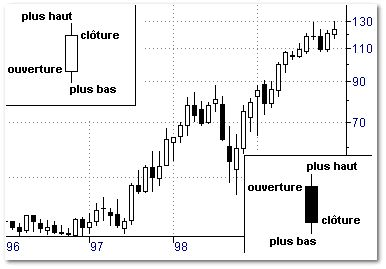
\includegraphics[scale=0.5]{../graph/chandelier.png}
  \caption{Exemple de graphique avec des chandeliers -\url{http://www.abcbourse.com/apprendre}}
\end{figure}

 La désignation pour le chandelier blanc (marché haussier) est le Yang (yo-sen ), pour le chandelier noir (marché baissier) le Yin (in-sen). \\
 
Normalement, après une bougie avec un corps long on ne doit pas prendre position sauf si on est dans un contexte haussier pour une bougie blanche ou contexte baissier pour une bougie noire. 

Pour effectuer des prévisions à partir des chandeliers, il faut être capable de repérer des figures significatives : 
\begin{itemize}
\item  \textbf{Ligne perçante} : représente un retournement. Un long corps de baisse suivi d’un long corps de hausse. Le trait horizontal représente le milieu de la bougie de baisse, la bougie de hausse doit clôturer au-dessus de ce trait.  
\begin{figure}[H]
  \center
  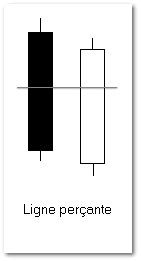
\includegraphics[scale=0.5]{../graph/chandelier1.png}
  \caption{Exemple de ligne perçante - \url{http://www.abcbourse.com/apprendre}}
\end{figure} 

\item \textbf{Ciel ouvert} : condition inverse de la ligne perçante. Un long corps de hausse suivi d’un long corps de baisse. Le corps de baisse ouvre au-dessus du milieu de la bougie de hausse. Ce motif représente un retournement également. 
\begin{figure}[H]
  \center
  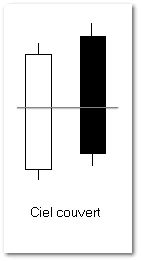
\includegraphics[scale=0.5]{../graph/chandelier2.png}
  \caption{Exemple de ciel ouvert - \url{http://www.abcbourse.com/apprendre}}
\end{figure} 

\item \textbf{Le marteau} : il présage d’une hausse si il arrive au cours d’une baisse. Il n’y a pas d’ombre au dessus et une très longue en dessous, il peut s’agir d’une bougie noire ou blanche la signification est la même .
\begin{figure}[H]
  \center
  
\includegraphics[scale=0.5]{../graph/chandelier3.png}
  \caption{Exemple de marteau - \url{http://www.abcbourse.com/apprendre}}
\end{figure} 

\item \textbf{Le pendu} : il présage d’une baisse si il arrive au cours d’une hausse. Les couleurs n’ont pas d’importance. 
 \begin{figure}[H]
  \center
  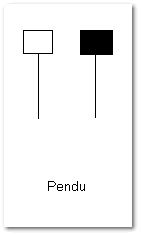
\includegraphics[scale=0.5]{../graph/chandelier4.png}
  \caption{Exemple de pendu - \url{http://www.abcbourse.com/apprendre}}
\end{figure} 

\item \textbf{Les englobantes} : Elles peuvent être haussières ou baissières et sont très puissantes. Si la baissière arrive après une hausse significative ou la haussière après une baisse significative, on assistera probablement à un retournement.
\begin{figure}[H]
  \center
  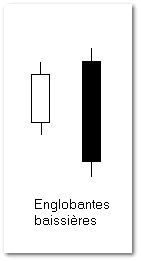
\includegraphics[scale=0.5]{../graph/chandelier5.png}
  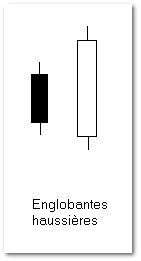
\includegraphics[scale=0.5]{../graph/chandelier6.png}
  \caption{Exemple d'englobante - \url{http://www.abcbourse.com/apprendre}}
\end{figure} 

\item \textbf{Étoile du soir et étoile du matin} : l’étoile du soir indique un retournement possible à la baisse et l’étoile du matin indique au contraire un retournement possible à la hausse.
\begin{figure}[H]
  \center
  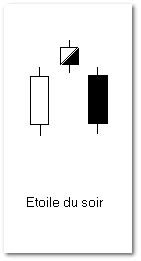
\includegraphics[scale=0.5]{../graph/chandelier7.png}
  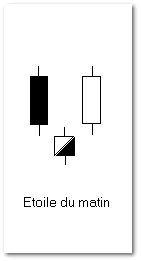
\includegraphics[scale=0.5]{../graph/chandelier8.png}
  \caption{Exemple d'étoile du soir et d'étoile du matin- \url{http://www.abcbourse.com/apprendre}}
\end{figure} 

\item \textbf{Les dojis} : Ils sont très simples à reconnaître : un seul trait horizontal indiquant que les cours de clôtures et d’ouvertures sont les mêmes. Il existe plusieurs types de doji. Le \textbf{doji simple} un long trait vertical de chaque côté de la barre horizontal indique de l’indécision. Les \textbf{dojis dragons}, sont composés d’un long trait sous la barre horizontale, les cours ont beaucoup baissés dans la journée pour se maintenir finalement. Le \textbf{doji pierre tombale} est l’inverse du doji dragon. Si plusieurs dojis se suivent : séance suivante très évolutive.
\begin{figure}[H]
  \center
  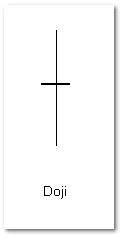
\includegraphics[scale=0.5]{../graph/chandelier9.png}
  
\includegraphics[scale=0.5]{../graph/chandelier10.png}
  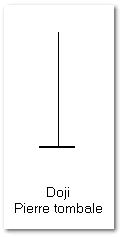
\includegraphics[scale=0.5]{../graph/chandelier11.png}  
  \caption{Exemple de dojis - \url{http://www.abcbourse.com/apprendre}}
\end{figure} 
\end{itemize}

\subsubsection{Les moyennes mobiles}
Les moyennes mobiles sont souvent cités mais pourtant souvent mises au second plan.  La Moyenne Mobile Arithmétique des cours de clôture calculée sur 20 jours, appelée MMA20 se calcule en additionnant les cours des 20 derniers jours et en divisant le résultat par 20. La MMA50, utilise le même principe mais pour 50 jours. Les pics de la courbe des moyennes mobiles sont retardés par rapport à la courbe du cours et sont plus aplatis et arrondis. 

\begin{figure}[H]
  \center
  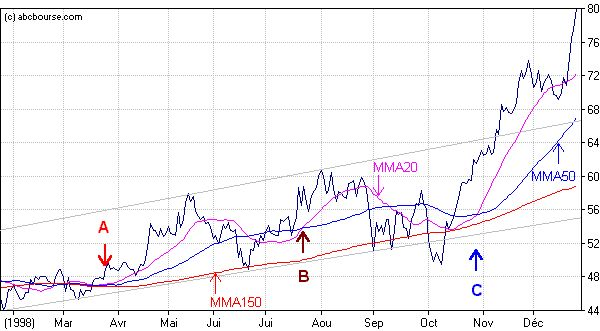
\includegraphics[scale=0.5]{../graph/moyennemobile.png} 
  \caption{Exemple de courbe avec moyenne mobile, en rose MMA20, en bleu MMA50 et en rouge MMA150 - \url{http://www.abcbourse.com/apprendre}}
\end{figure} 

Seule une MMA ne nous donne que très peu d’information, mais en étudiant deux courbes de moyenne mobile on peut en déduire des points intéressants. Lorsque la courbe de la MMA de moyenne la plus courte vient couper la courbe de la MMA de moyenne la plus longue en passant par dessus, la valeur entame un cycle de hausse. Lors d'un croisement entre deux MMAs le gain potentiel est plus fort si l’angle entre les deux MMAs est plus important. \\

Il est conseillé d'effectuer le choix suivant : la MMA de durée longue doit avoir une durée entre deux et quatre fois plus longue que la durée courte, on associe souvent MMA20 et MMA50

Il existe des contre-exemple connus au moyenne mobile :
\begin{itemize}
\item échange de quelques actions par jour seulement, lorsqu'il y a possibilité que les achats par jour puissent faire changer significativement la moyenne mobile de durée courte
\item des actions indépendantes du marché, il ne faut pas prendre MMA20 et MMA50 mais d'autres durée pour coller au titre
\end{itemize}

Il existe d'autres types de moyenne mobile, tels que les Moyennes Mobiles Exponentielles définies par la formule suivante : \\
$MME = Moyennes Mobiles Exponentielles = fermeture du jour * 0.09 + MM de la veille * 0.91$. 


\subsubsection{Les Bandes de Bollinger}
Les Bandes de Bollinger ont été inventées dans les années 80 par John Bollinger. C'est désormais un des indicateurs classiques en analyse technique.  Il sert à évaluer l'évolution future du prix d'un cours. Les Bandes de Bollinger déterminent les niveaux de résistance à la hausse et de support à la baisse. \\

Étudions dans un premier temps la construction des bandes de Bollinger. Dans un premier temps il nous faut une Moyenne Mobile sur n périodes (en général n=20). Cette courbe est appelée la Moyenne Mobile de Bollinger. La Bande Supérieure de Bollinger est calculée de la manière suivante : notre Moyenne Mobile de Bollinger, défini précédemment, plus un nombre x fois écart-types des cours avec cette Moyenne Mobile(en général x=2). La Bande Inférieure de Bollinger est déterminée d'une manière analogue : notre Moyenne Mobile de Bollinger moins x fois écart-types des cours avec cette Moyenne Mobile. \\

L'écart-type est calculé de la manière suivante : $ecartType= \sqrt{\sum{\frac{(cloture-MMS)^2}{n}}} $ \\

Les Bandes de Bollinger sont ainsi deux courbes placées à égales distance de la Moyenne Mobile, elles forment un canal. On peut voir leur représentation sur le schéma suivant, en bleu nous retrouvons la Moyenne Mobile de Bollinger alors qu'en rouge nous retrouvons les deux bandes de Bollinger : 

\begin{figure}[H]
  \center
  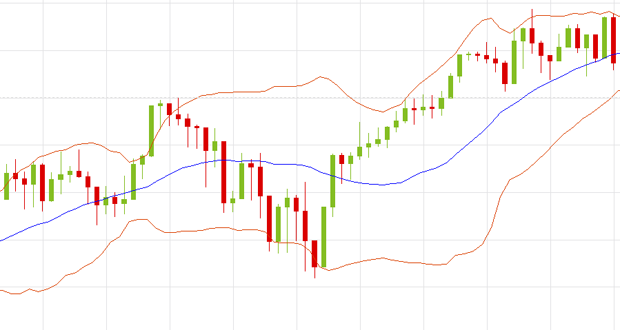
\includegraphics[scale=0.5]{../graph/bollinger.png} 
  \caption{Exemple de bande de Bollinger - \url{https://www.forexagone.com/apprendre/bandes-bollinger}}
\end{figure} 

Maintenant que nous avons défini les Bandes de Bollinger, étudions les informations que nous apportent ces bandes. \\

Première approche avec les Bandes de Bollinger : lorsqu'une tendance est clairement définie, il faut entrer en action lorsque le cours dépassera la bande de Bollinger. Dans le cas d'une tendance haussière, il faudra regarder quand le cours débordera la Bande Supérieure de Bollinger et inversement en tendance baissière il faudra regarder par rapport à la Bande Inférieure de Bollinger. Ainsi dans l'exemple ci-dessous, nous sommes clairement dans le cas d'une tendance baissière. Nous remarquons que le cours franchit trois fois la Bande Inférieure de Bollinger, sur cet exemple il aurait fallu prendre des positions vendeuses à trois reprises. 

\begin{figure}[H]
  \center
  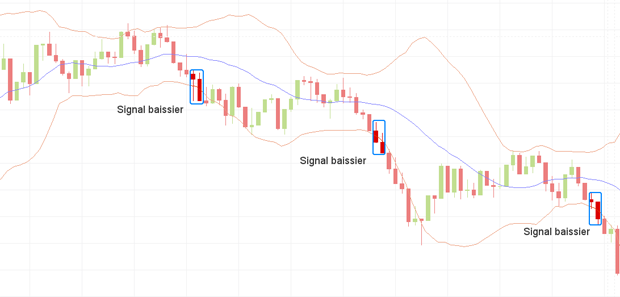
\includegraphics[scale=0.5]{../graph/bollingerBaissier.png} 
  \caption{Exemple de bande de Bollinger en tendance baissière - \url{https://www.forexagone.com/apprendre/bandes-bollinger}}
\end{figure} 
 
 
Deuxième situation : Lorsque le cours n'a pas de tendance clairement défini, il faut faire attention au moment ou le cours croise une Bande de Bollinger. En effet, lorsque le cours croise la Bande Supérieure de Bollinger il faut vendre car les prix vont diminuer et inversement lorsque le cours va toucher la Bande Inférieur il faut acheter. Nous pouvons voir cela sur l'exemple ci-dessous, chaque flèche verte représente un moment où il faut acheter car le cours atteint la Bande Inférieure. Les flèches rouges quand à elles représentent les moments où il faut vendre car le cours atteint la Bande Supérieure.  

\begin{figure}[H]
  \center
  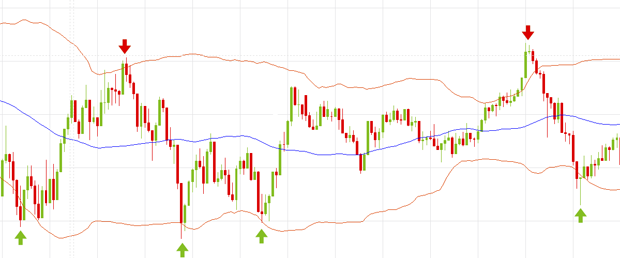
\includegraphics[scale=0.5]{../graph/bollingerRange.png} 
  \caption{Exemple de bande de Bollinger sans tendance - \url{https://www.forexagone.com/apprendre/bandes-bollinger}}
\end{figure} 
 
La dernière situation dans laquelle les Bandes de Bollinger sont utiles est la suivante : lorsque les bandes de Bollinger se ressert très fortement, on appelle cette situation un étranglement. Lorsque l'on est dans le cas d'un étranglement la volatilité des prix est très faible, en effet l'écart-type est très faible ce qui amène le resserrement des deux bandes. Ces phases d'étranglement sont le signe d'une phase d'accélération du cours et donc de volatilité très importante. Les bandes de Bollinger ne nous permettent pas de savoir dans quelle directions les cours vont varier, il faudra dont utiliser d'autres méthodes pour compléter cette analyse et déterminer la tendance qui va suivre. Dans l'exemple ci-dessous nous pouvons remarquer un étranglement dans la zone encadrée en bleue : la volatilité est très faible. Nous savons donc qu'il va y avoir une forte variation du cours à venir. Cela se vérifie lorsque le cours croise la bande inférieure de Bollinger : il s'en suite une chute importante.   

\begin{figure}[H]
  \center
  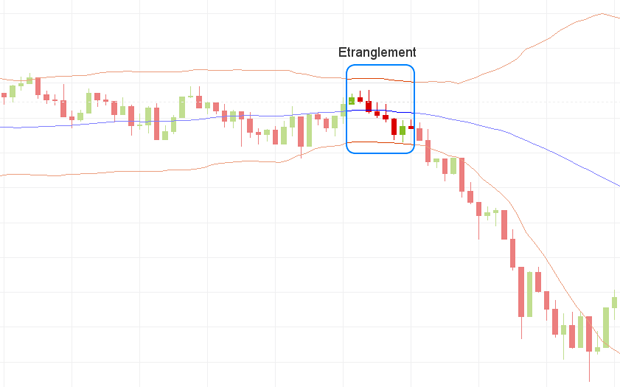
\includegraphics[scale=0.5]{../graph/bollingerEtranglement.png} 
  \caption{Exemple de bande de Bollinger avec étranglement - \url{https://www.forexagone.com/apprendre/bandes-bollinger}}
\end{figure} 
 
Les bandes de Bollinger présente l'avantage d'être très réactif car il sait prévoir les grands changement à venir pour le cours. Néanmoins, il présente l'inconvénient d' évoluer rapidement d'une séance à l'autre. Leur interprétation doit donc être réalisée fréquemment afin d'éviter des erreurs de jugements.  

\subsubsection{Les volumes}
Les volumes correspondent au nombre de titre échangé sur une unité de temps pour un titre. Dans notre cas l'unité de temps sera toujours la journée. L'étude des volumes peut nous apporter beaucoup de connaissances sur un cours, par exemple sur sa tendance ou sur la force de sa résistance ou se son support. C'est un très bon indicateur de la situation du marché. \\

Tout d'abord, étudions les différentes parties pour représenter les volumes sur un graphe. Il en existe deux principales. La première façon, la plus répandue est de représenter sous forme de traits verticaux en dessous des cours. Nous pouvons le voir dans l'exemple ci-dessous : 

\begin{figure}[H]
  \center
  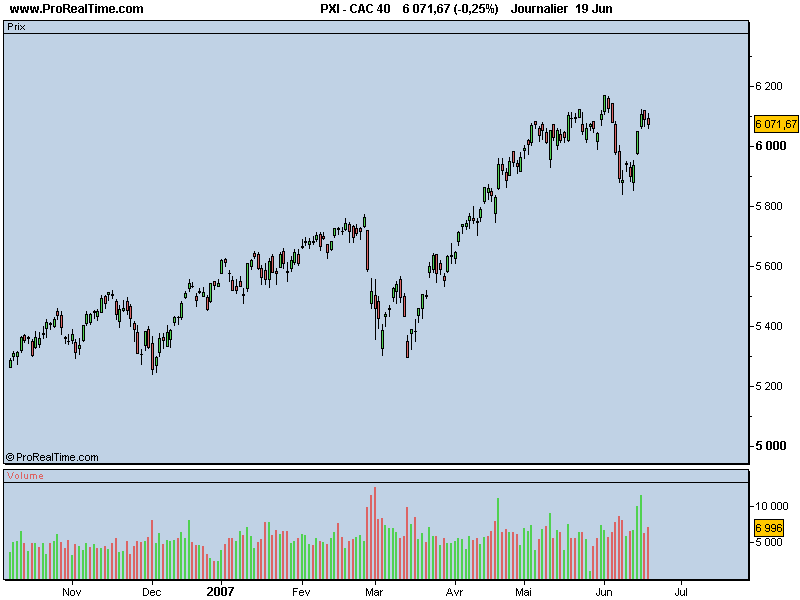
\includegraphics[scale=0.5]{../graph/volumeBarre.png} 
  \caption{Représentation du volume par niveau de prix - \url{http://www.trading-school.eu/glossaire-bourse/}}
\end{figure} 

La deuxième façon de représenter le volume est par niveau de prix. Sur le graphique ci-dessous, nous voyons les volumes comme étant les barres horizontales sur la gauche du graphique. Cette façon de représenter les volumes possède l'avantage de clairement faire apparaître le support et la résistance. 

\begin{figure}[H]
  \center
  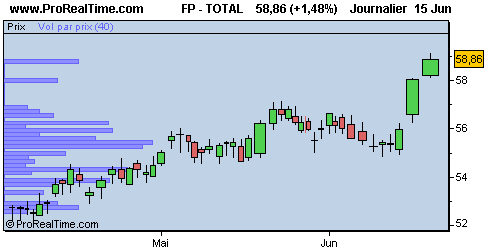
\includegraphics[scale=0.5]{../graph/volumePrix.png} 
  \caption{Exemple de représentation du volume - \url{http://www.trading-school.eu/glossaire-bourse/}}
\end{figure}  

Une fois que nous avons étudier la façon de représenter les volumes, étudions quelles informations nous pouvons en tirer. En effet, une modification des volumes peut-être le signe d'un changement de situation dans le marché. \\

Une tendance haussière est considérée comme saine lorsqu' il y a une augmentation des volumes en simultanés. De préférence, il faut que les volumes soient en hausse lorsque de nouveaux plus hauts sont atteints. En effet, cela prouve une véritable attraction de la part des investisseurs pour ce titre. Une hausse des prix sans augmentation des volumes est due à un faible nombre d'acheteur et pourrait être totalement contrariée par un grand nombre de vendeur. Après une forte augmentation des cours ininterrompues conjuguées à une forte augmentation des volumes il faut être prudent car il risque de ne plus y avoir d'acheteurs et un grand nombre de vendeurs peut venir contrarier cette tendance. 

Dans une tendance baissière il n'y a besoin de forts volumes pour constater une forte baisse du prix. C'est le cas dans un marché où il y a de nombreux vendeurs et peu d'acheteurs. En revanche, de faibles volumes n'implique pas forcément une baisse du cours. Attention cependant au phénomène de Sell-off qui correspond à une baisse significative des cours accompagnés de forts volumes. Ce phénomène est en général le signe de la fin d'une baisse car tous les titres sont vendus à n'importe quel prix. 
	
	\section{Gestion de portefeuille}


\subsection{Définitions et généralités}

Un \textbf{portefeuille} est un ensemble homogène de ressources ou d'actifs. En finance, un portefeuille est composé d'actfis financiers qui peuvent être de différentes natures (actions, obligations, options,...).\\

\noindent La \textbf{gestion de portefeuille} consiste à :
\begin{itemize}
 \item Gérer des capitaux tout en respectant les contraintes réglementaires et contractuelles qu'on peut avoir.
 \item Appliquer les politiques d'investissements définies au départ par le propriétaire du portefeuille.
 \item Tirer le meileur rendement possible en fonction du niveau de risque choisi par l'investisseur.\\
\end{itemize}

\noindent Afin d'illuster la gestion de portefeuille en général et sans rentrer tout de suite dans le cadre de la gestion d'un portefeuille d'actifs financiers, voyons les exemples suivants qui illustrent différents objectifs :
\textit{
\begin{enumerate}
 \item Un individu seul voudra par exemple préparer sa retraite ou bien simplement investir en bourse plutôt que laisser son argent dormir sur un compte qui rapport peu.
 \item Les banques elles auront pour but de faire fructifier les dépôts de ses clients pour pouvoir verser les intérêts et surtout avoir suffisamment de liquidités en cas de retraits massifs de ces même dépôts.
 \item Les assureurs quant à eux auront pour objectifs d'assurer le paiement des sinistres et, en cas de situations exceptionnelles, ils auront besoin de liquidités (exemple : catastrophe naturelle).
\end{enumerate}
}

\subsubsection{Les différents risques}
On identifie deux grands types de risques lorsque l'on investi dans un portefeuille d'actifs financiers :
\begin{enumerate}
 \item \textbf{Les risques financiers :} lorsque l'on investi sur les marchés financiers, on est par définition exposé aux risques qu'ils comportent.
    \begin{itemize}
     \item \underline{Le risque de marché :} il existe une incertitude en ce qui concerne les taux de marché, les prix des actifs (actions, devises,...).
     \item \underline{Le risque de crédit, de contrepartie, de défaut :} on n'est pas à l'abri du fait que la personne en face remplisse ses obligations, sauf si l'on est dans le cadre d'un marché organisé.
     \item \underline{Le risque de liquidité :} il est possible qu'on soit obligé de vendre un actif à un prix plus faible que sa juste valeur, on perd alors de l'argent.
    \end{itemize}
 \item \textbf{Les risques non-financiers :} il en existe énormément, nous ne citerons que ceux qui peuvent vraiment avoir un impact dans la situtation d'un individu qui investi seul (et non pas la gestion d'un portefeuille pour une entreprise telle qu'une banque ou un assureur).
    \begin{itemize}
     \item \underline{Le risque de modèle :} on peut se tromper de modèle d'évaluation des actifs, d'analyse ou d'aide à la décision.
     \item \underline{Le risque de liquidité :} il est possible qu'on soit obligé de vendre un actif à un prix plus faible que sa juste valeur, on perd alors de l'argent.
     \item \underline{Le risque de perte extrême :} c'est par exemple le risque qu'une entreprise pourtant très solide s'effondre.
    \end{itemize}
\end{enumerate}
Il est important de préciser que les risques ne sont pas indépendants, c'est pourquoi il faut être d'autant plus vigilant.

\subsubsection{Processus de gestion d'un portefeuille}
On peut établir un processus de gestion d'un portefeuille, il est généralement utilisé en entreprise mais on peut l'adapter à n'importe quel investisseur :
\begin{enumerate}
 \item \textbf{Planifier :} comprendre les besoins de l'investisseur, analyser sa tolérance au risque et préparer une politique de placement (objectifs, contraintes).
 \item \textbf{Exécuter :} allouer des actifs au portefeuille, les analyser et construire le portefeuille.
 \item \textbf{Faire un bilan :} mesurer les performances du portefeuille et le modifier ou l'ajuster en fonction des résultats.
\end{enumerate}

\subsubsection{La diversification d'un portefeuille}
Diversifier son portefeuille est la première chose à faire lorsque l'on souhaite éviter le risque de perte du capital investi. On peut justifier ceci à l'aide de l'exemple suivant :

\paragraph{Exemple :} \textit{Un individu qui investi dans une seule entreprise depuis 10 ans pour préparer sa retraite, le cours de l'action ne fait qu'augmenter, mais il peut arriver que l'entreprise subisse un 'coup dur' et alors son cours va chuter de manière rapide et critique. L'individu aura alors tout perdu.
	  S'il avait investi dans un portefeuille, il aurait été peu probable que tous ses actifs chutent en même temps (sauf en cas de crise économique répandue) et la chute d'une entreprise aurait eu des conséquences moindres sur son investissement.}
	  \begin{figure}[H]
	    \center
	    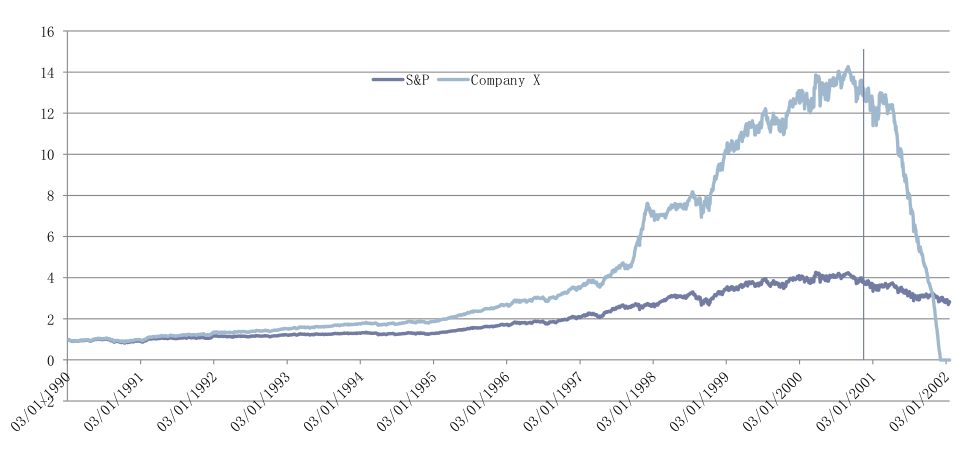
\includegraphics[scale=0.4]{../graph/exempleChuteEntreprise.png} \\
	    \caption{Exemple fictif d'une entreprise dont le cours augmente pendant de nombreuses années jusqu'au moment où le cours chute brutalement. La courbe bleue foncée représente un indice contenant l'entreprise X.}
	  \end{figure}
	  
L'exemple précédent mène à deux conclusions importantes : diversifier son portefeuille permet d'éviter les catastrophes et de réduire le risque sauf dans certains cas. En effet, en cas de crise économique, tous les actifs deviennent plus ou moins corrélés et chutent en même temps. Dans ce cas, on observerait probablement une chute générale des actifs du portefeuille comme on peut le voir sur le graphe suivant par exemple :
	  \begin{figure}[H]
	    \center
	    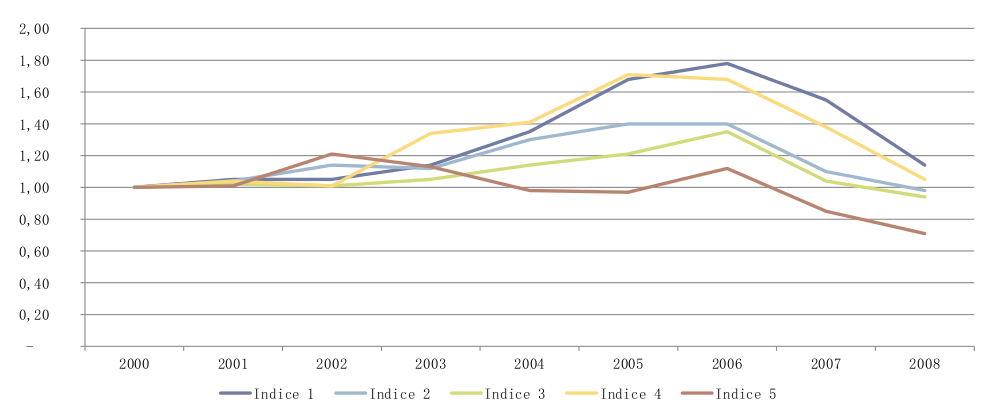
\includegraphics[scale=0.4]{../graph/exemplePortefeuilleChute.png} \\
	    \caption{Exemple fictif d'un portefeuille dont les actifs n'étaient au départ pas corrélés mais qui a la fin de 2006 ont tous chutés en même temps du fait de la crise.}
	  \end{figure}
Nous allons voir par la suite qu'un investissement est caractérisé par son rendement et sa volatilité (c'est-à-dire son rique).

\subsubsection{Les différents profils de risque}
Si l'on pose la question suivante à une population d'individus, on aura trois types de réponses :\\

\textit{Que choisissez-vous si l'on vous propose :
\begin{enumerate}
 \item Gagner 1 000\euro\ de manière certaine.
 \item Gagner 2 000\euro\ avec une chance sur deux.
\end{enumerate}
}
\noindent Dans les deux cas l'espérance de gain est de 1 000\euro\ . Voyons les différents types de réponse que l'ont peut avoir :
\begin{itemize}
 \item \underline{Les risk lovers/seekers :} ces personnes aiment le risque et auront tendance à choisir la deuxième possibilité.
 \item \underline{Les risk neutral :} ce sont les individus indécis. Souvent, ils regardent uniquement l'espérance de rendement et ne s'occupent pas vraiment du risque. Du coup, il ne savent pas choisir entre les deux propositions.
 \item \underline{Les risk adverse :} cette catégorie de personnes choisira la première solution sans hésiter puisque ce sont des individus averses au risque, il le fuit et veulent avoir un gain sûr minimal.
\end{itemize}
Bien sûr, nous nous sommes basé sur un exemple subjectif, le choix des personnes ne sera sans doute pas le même si l'on augmente le gain potentiel (100 000\euro\ ou 200 000\euro\ par exemple). En effet, on verra que beaucoup de personnes qui avaient choisi la deuxième possibilité ou étaient indécis vont alors choisir le premier choix. Cette notion dépend donc du capital de chaque individu. Néanmoins, cela donne une idée de la tolérance au risque de la personne. 

\subsubsection{La classification des actifs selon leur risque}
On distingue les actifs risqués des actifs moins risqués voir même des actifs dits 'sans risque'.
\begin{itemize}
 \item \textbf{Actifs 'sans risque' :} produits monétaires (prêts interbancaires, change à terme, swaps de taux d'intérêt, swaptions,...).
 \item \textbf{Actifs peu risqués :} ce sont les obligations, les emprunts d'Etats ou d'entreprise bien notée (de AAA à BBB).
 \item \textbf{Actifs risqués :} les obligations convertibles puis les actions.
 \item \textbf{Actifs très risqués :} les produits dérivés en général.
\end{itemize}
\begin{figure}[H]
  \center
  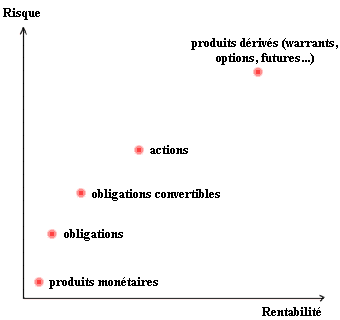
\includegraphics[scale=0.6]{../graph/actifsRisques.png}
  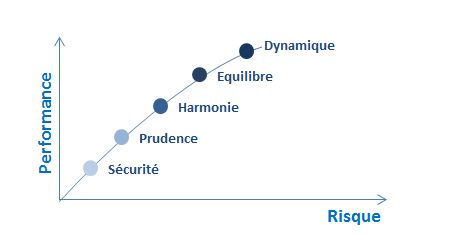
\includegraphics[scale=0.6]{../graph/profilsRisque.png}
  \caption{Graphe Risque/Rendement des différents types d'actifs - \url{http://www.abcbourse.com/apprendre/4_constituer_un_portefeuille2.html}}
\end{figure}


\subsection{L'évaluation d'un actif financier}
Un actif financier a la particularité de pouvoir être représenté par son rendement et son risque (ou volatilité). Nous allons donc voir comment les calculer.

\subsubsection{Le rendement}
Il existe deux types de rendements :
\begin{itemize}
 \item Les rendements périodiques/ponctuels : les dividendes, les coupons, les intérêts,...
 \item Les rendements continus : appréciation et dépréciation des actifs. On appelle cela le Profit \& Loss (P\&L), c'est le gain ou la perte en capital.
\end{itemize}

Il existe différentes manières de calculer le rendement d'un actif :
\begin{enumerate}
 \item \textbf{Le rendement Holding Period (sur la période de détention) :} c'est la différence entre le prix à la fin de la période et le prix au début, sommé avec les dividendes et le tout divisé sur le prix de départ.
 \[ R_{Holding Period} = \frac{Prix_{Fin}-Prix_{Debut}+dividendes}{Prix_{Debut}} \]
 En réalité cela donne un taux de rendement. Si on a invesit 1\euro\ au départ, on aura à la fin de la période \((1 + R_{Holding Period})\times 1\)\euro.
 \item \textbf{Le rendement arithmétique (ou moyen) :} c'est la moyenne des rendements $R_i$ sur plusieurs périodes.
 \[ R_{i} = \frac{1}{T} \sum_{t=1}^T R_{i,t}\]
 \item \textbf{Le rendement géométrique :} il est plus proche de la réalité que le rendement arithmétique qui lui fausse la vision que l'on a sur le vrai rendement.
 \[ R_{i} = \sqrt[T]{\prod_{k=1}^{T}(1+R_{i,k})}-1\]
 \item \textbf{Le Taux de Rendement Interne (TRI) :} c'est le taux d'actualisation qui annule la valeur actuelle nette (VAN) de la série des cash flows (flux de trésorerie).
 \[ VAN = \sum_{t=0}^{T} \frac{CashFlow}{(1+TRI)^t} = 0\]
 \item \textbf{Le rendement annualisé :} c'est le rendement d'une période ramené à un an.
 \[ R_{annuel} = (1+R_{periode})^C\]
 où $C$ est le nombre de périodes par an.
\end{enumerate}
Il existe d'autres types de rendements que nous ne détaillerons pas comme le rendement nominal avant ou après taxe.\\

Maintenant que l'on est capable de calculer le rendement d'un actif, on peut calculer le rendement d'un portefeuille composé de plusieurs actifs. Pour cela on définit les poids de chaque actifs $w_i$ et les rendements de chaques actifs $R_i$. Alors le rendement du portefeuille $R_P$ vaut :
\[ R_P = \sum_{i=1}^{N}w_iR_i\]
avec $N$ le nombre d'actifs différents du portefeuille et la somme des poids qui vaut 1 : \(\sum_{i=1}^{N}w_i =1\).

\subsubsection{La volatilité}


%Exemple bidon :
%Même rendement et volatilités différentes : on choisit la volatilité la plus faible si on est censé.
%Même volatilité et rendements différents : meilleur rendement.


%Analyse d'un historique : variance (volatilité)
%Covariance entre deux actifs
%Optimisation d'un portefeuille : Markowitz


%la VaR?

\subsection{La théorie moderne du portefeuille}

	
	\section{Introduction}

	
	
\chapter{Modélisation}
	\section{Description générale du modèle}

\subsection{Cas d'utilisation}
Voici le diagramme des cas d'utilisation que nous avons choisi et qui définira par la suite certaines contraintes de notre modèle :\\

\begin{figure}[H]
  \center
  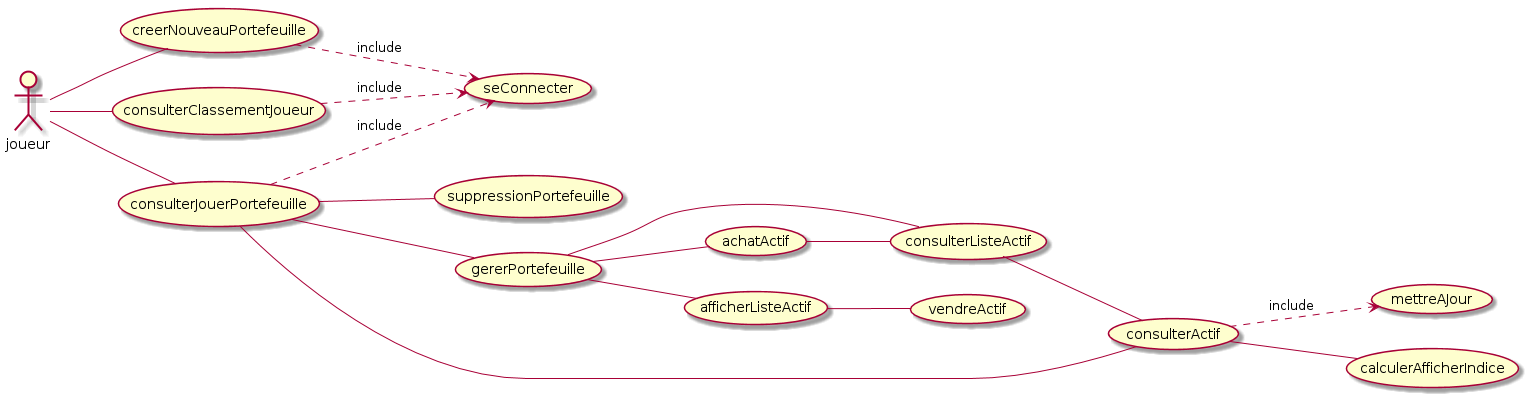
\includegraphics[scale=0.35]{../graph/CasDutilisationGeneral.png} 
\end{figure}

Un joueur peut : créer un nouveau portefeuille, consulter l'état du jeu (i.e. le classement des joueurs) ou encore consulter et jouer avec son portefeuille, sous réserve qu'il se soit connecté au préalable. \\ \\
Lorsqu'il choisit de consulter et jouer avec son portefeuille, quatre options s'offrent à lui : il peut consulter un actif précis, consulter la liste des actifs côtés s'il ne sait pas exactement ce qu'il cherche, gérer son portefeuille et jouer, ou encore supprimer son portefeuille afin de stopper la partie. \\ \\
Si le joueur consulte un actif, la bourse sera mise à jour avant qu'il ne puisse éventuellement récupérer un indicateur technique sur ce titre.\\ \\
Si le joueur consulte la liste des actifs, il pourra alors en sélectionner un et se retrouvera dans le cas précédent. \\ \\
Si le joueur choisit de gérer son portefeuille, il peut consulter la liste des actifs de la bourse (et se retrouvera dans la situation précédente), il peut aussi acheter un actif en parcourant la bourse (liste des actifs), et sa dernière possibilité consiste en la consultation des actifs présents dans son portefeuille avant de pouvoir, s'il le souhaite, en vendre une partie.

	
	\section{Différents package}

\begin{figure}[H]
  \center
  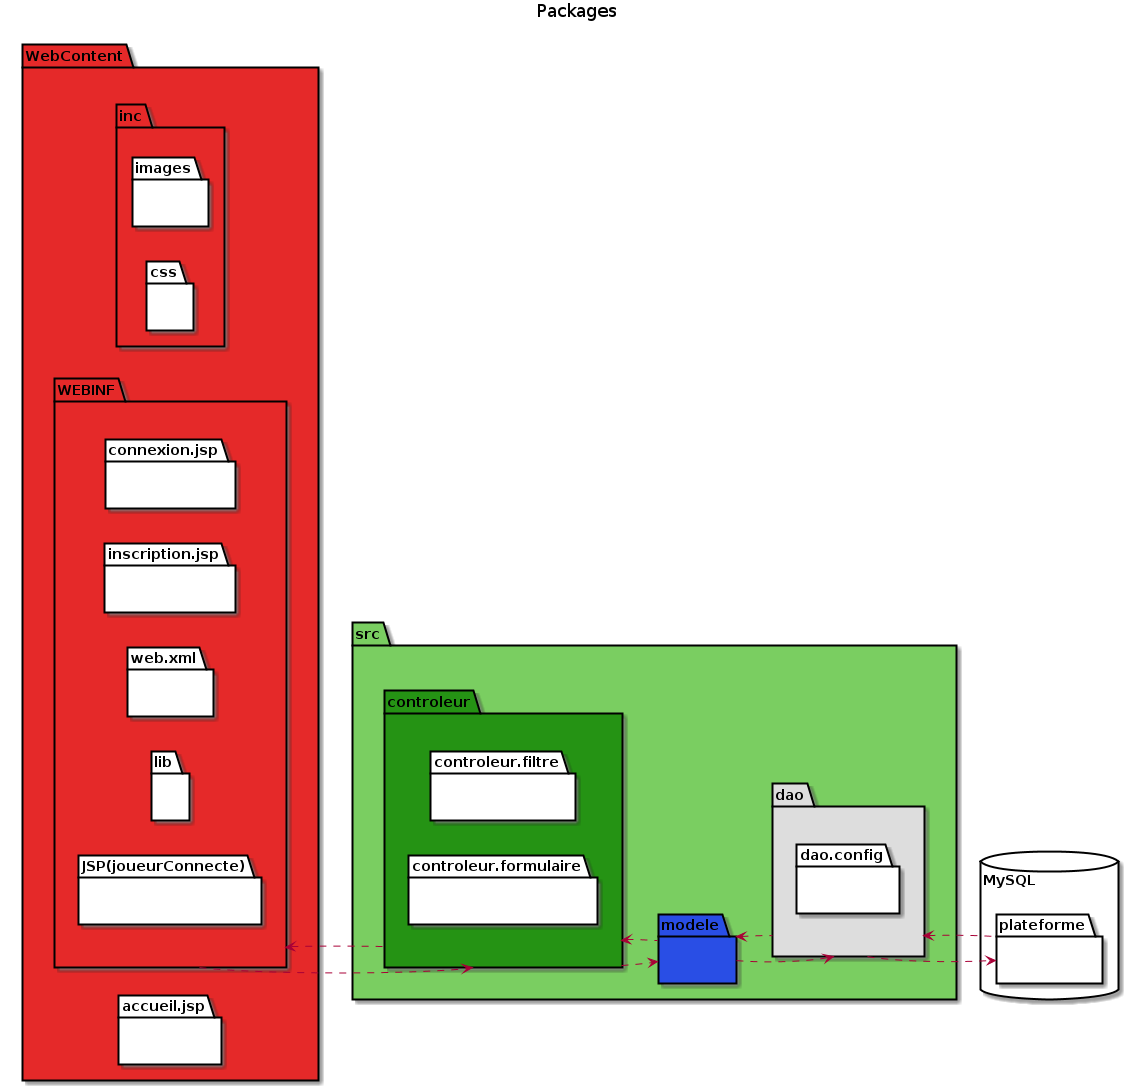
\includegraphics[scale=0.25]{../graph/packages.png} \\
  \caption{Vue d'ensemble des packages}
\end{figure}

\begin{figure}[H]
  \center
  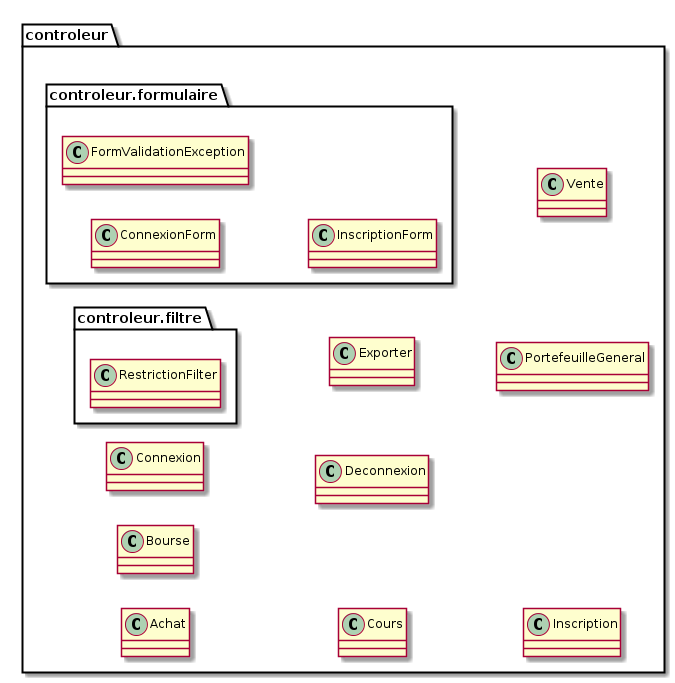
\includegraphics[scale=0.25]{../graph/packageControleur.png} \\
  \caption{Package Controleur}
\end{figure}

\begin{figure}[H]
  \center
  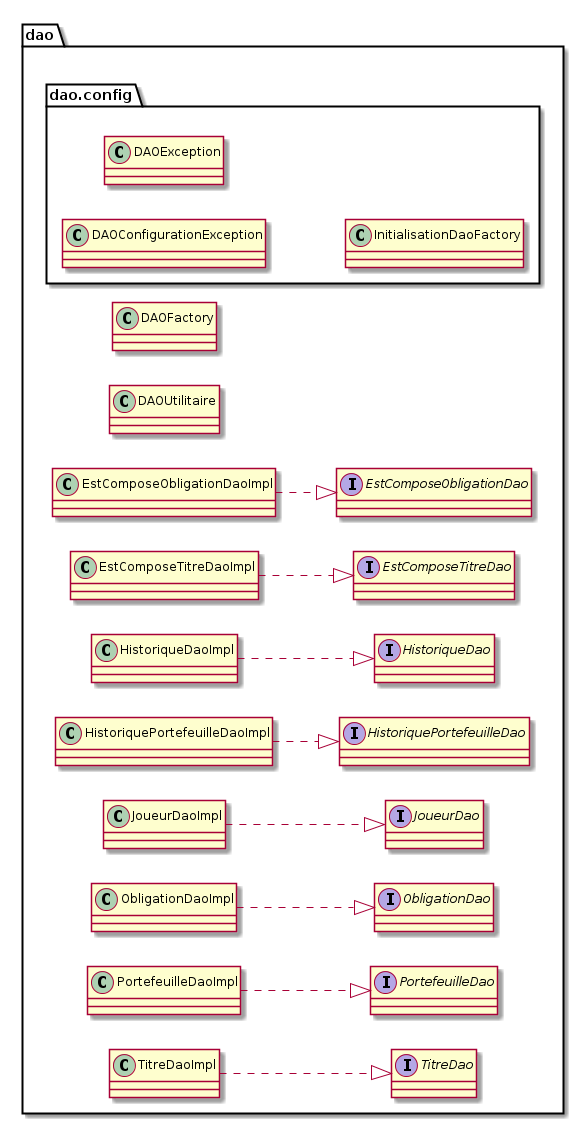
\includegraphics[scale=0.25]{../graph/packageDAO.png} \\
  \caption{package Dao}
\end{figure}

	
	\section{Diagramme de classe}

\begin{figure}[H]
  \center
  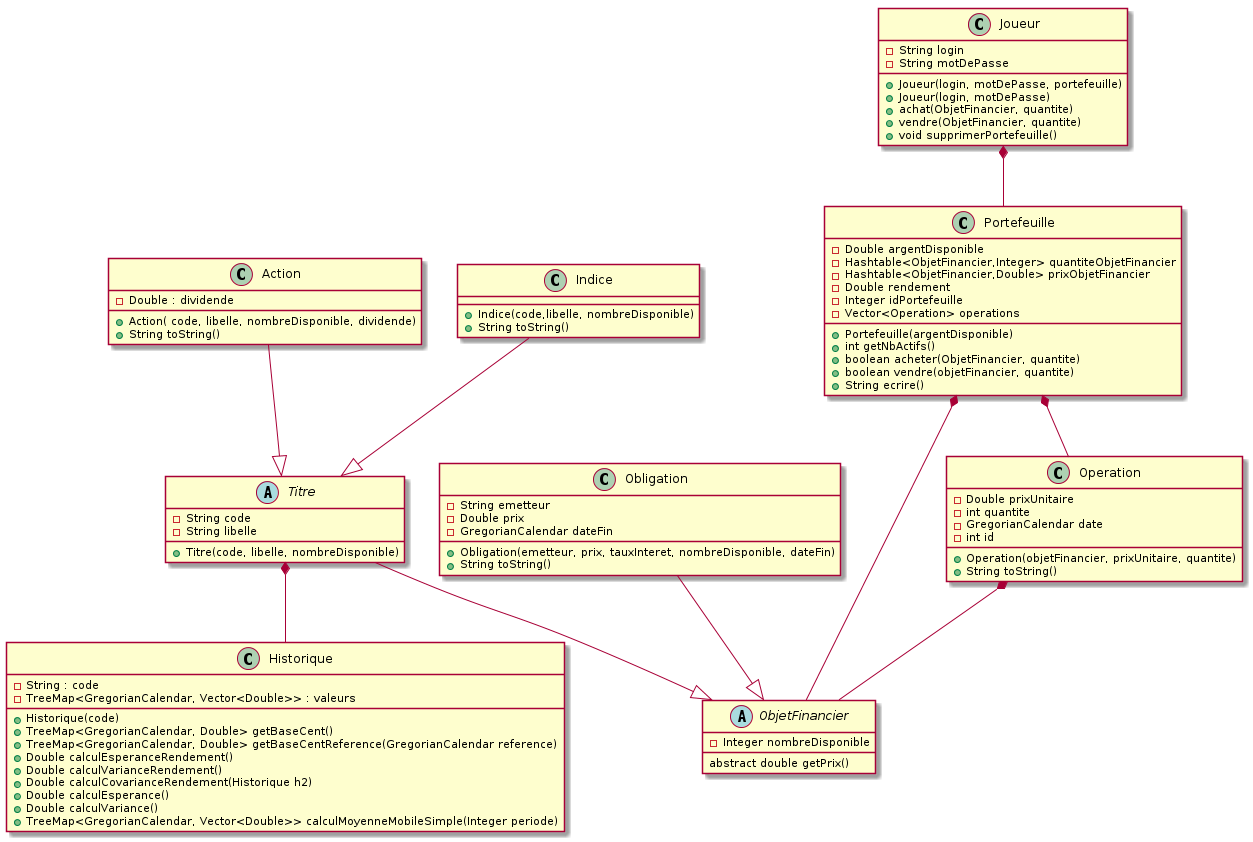
\includegraphics[scale=0.25]{../graph/DiagrammeClasseFinalModele.png} \\
  \caption{Diagramme de classe}
\end{figure}

	
	\section{Diagramme de séquence }

Nous avons choisi de proposer les diagrammes de séquence des parties les plus importantes de notre projet. 

\subsection{Inscription}
\begin{figure}[H]
  \center
  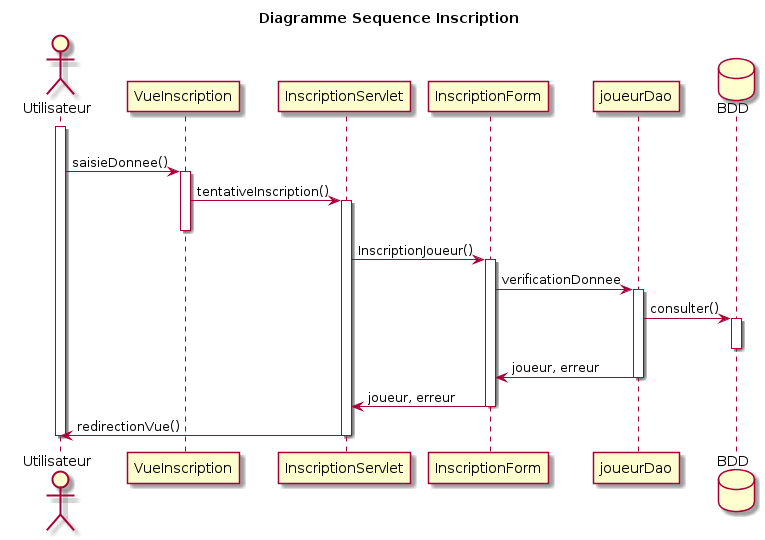
\includegraphics[scale=0.35]{../graph/DiagrammeSequenceInscription.png} \\
  \caption{Diagramme de séquence inscription}
\end{figure}

Ce diagramme correspond à l'inscription. L'inscription commence par la saisie du login et du mot de passe par l'utilisateur. Ensuite le formulaire d'inscription vérifie les données en entrée (login assez long et non utilisé, les deux mots de passe identiques). Si les données entrées sont correctes, l'utilisateur est alors ajouté à la base de donnée, avant d'ajouter le joueur dans la table on encrypte son mot de passe grâce à Jasypt. Si les données ne sont pas correctes, on renvoie un message d'erreur à l'utilisateur. 

\subsection{Connexion}
\begin{figure}[H]
  \center
  \includegraphics[scale=0.35]{../graph/DiagrammeSequenceConnexion.png} \\
  \caption{Diagramme de séquence connexion}
\end{figure}

Ce diagramme correspond à la connexion. Le principe est le même que pour l'inscription : le joueur saisie les données (login, mot de passe). Elles sont ensuite vérifiées par le formulaire de connexion. Si les données sont correctes le joueur est connecté et ajouté en session. L'utilisateur a ainsi accès a de nouvelles pages.

\subsection{Achat Actif}
\begin{figure}[H]
  \center
  \includegraphics[scale=0.35]{../graph/DiagrammeSequenceAchatActif.png} \\
  \caption{Diagramme de séquence achat actif}
\end{figure}

Ce diagramme représente le diagramme de séquence général pour l'achat d'un objet financier. L'utilisateur choisit un actif qu'il veut acheter et choisit une quantité. Ensuit la servlet lance la méthode acheter du Joueur qui renvoie vraie si l'achat est réussi (argent disponible suffisant, quantité disponible de l'objet financier supérieur à la quantité demandée) et faux si l'achat échoue. Si l'achat est réussi on met à jour la base de donnée, s'il n'est pas réussi on renvoie un message d'erreur à l'utilisateur. 

\subsection{Achat Actif - Modele}
\begin{figure}[H]
  \center
  \includegraphics[scale=0.35]{../graph/DiagrammeSequenceAchatActifModele.png} \\
  \caption{Diagramme de séquence achat actif - Modele}
\end{figure}

Ce diagramme de séquence correspond à un zoom de ce qu'il se passe lors de l'achat d'un actif dans le modèle. Lors de l'achat d'un actif, le joueur appelle la méthode acheter du portefeuille. Le portefeuille vérifie d'abord que la quantité disponible est suffisante, ensuite que le joueur possède assez d'argent. Si les deux conditions précédentes sont réunies, on met à jour le prix de l'objet financier (moyenne pondéré avec l'ancien prix et les quantités), on met à jour la quantité de l'objet (simple addition) ainsi que l'argent disponible et le rendement du portefeuille. 

\subsection{Vente actif}
\begin{figure}[H]
  \center
  \includegraphics[scale=0.35]{../graph/DiagrammeSequenceVenteActif.png} \\
  \caption{Diagramme de séquence vente actif}
\end{figure}

Ce diagramme de séquence correspond au diagramme de séquence de la vente d'un actif. Le principe est le même que pour l'achat d'un actif c'est à dire que l'utilisateur choisit un actif et une quantité. On vérifie que la quantité d'actif que le joueur possède est supérieure à la quantité d'actifs qu'il souhaite vendre. Enfin, si c'est le cas on effectue la vente et on met à jour la base de données. Si ce n'est pas le cas, on lui renvoie un message d'erreur.  

\subsection{Supprimer portefeuille}
\begin{figure}[H]
  \center
  \includegraphics[scale=0.3]{../graph/DiagrammeSequenceSupprimerPortefeuille.png} \\
  \caption{Diagramme de séquence supprimer Portefeuille}
\end{figure}

La dernière opération principale que peut réaliser un joueur est la suppression de son portefeuille. Lors de la suppression du portefeuille, il faut supprimer toutes les lignes qui correspondent au portefeuille dans la base de données : il faut faire attention à l'ordre pour ne pas avoir de problèmes avec les clés lointaines. Nous supprimons donc d'abord les lignes dans EstComposeTitre et EstComposeObligation ensuite dans HistoriquePortefeuille qui correspond à l'historique des opérations et enfin dans la table Portefeuille. On attribue au joueur un nouveau portefeuille avec 10000 euros comme au début du jeu. 
	
	
\begin{frame}
    \frametitle{portefeuille}
  

\end{frame}
	
	
\begin{frame}
    \frametitle{Présentation}
    \begin{block}{Définitions}
	\begin{itemize}
	\item \textbf{Gestion de portefeuille :}
	      \begin{itemize}
	      \item Gérer des capitaux sous certaines contraintes
	      \item Choisir une stratégie d'investissement
	      \end{itemize}
	\item \textbf{Différents risques :}
	      \begin{itemize}
	      \item Financiers : marché, crédit, liquidité
	      \item Non financiers : modèle, perte extrême
	      \end{itemize}
	\item \textbf{Profils de rique :}
	      \begin{itemize}
	      \item Risk adverse
	      \item Risk neutral
	      \item Risk lovers/seekers
	      \end{itemize}
	\end{itemize}
    \end{block}


\end{frame}

\begin{frame}
    \frametitle{Actifs risqués}
	  \begin{figure}
	      \includegraphics[scale=0.5]{images/actifsRisques.png}   
	  \end{figure}   
\end{frame}


\begin{frame}
    \frametitle{Diversification} 
      \begin{block}{Intérêts}
	\begin{enumerate}
	  \begin{columns}
	    \begin{column}{4cm}
	      \item Eviter les catastrophes
	    \end{column}
	    \begin{column}{4cm}
	      \item Réduire le risque	   
	    \end{column}
	  \end{columns}
	\end{enumerate}
      \end{block}
      \begin{figure}
	  \includegraphics[scale=0.2]{images/exempleChuteEntreprise.png}   
	  \caption{Exemple d'un portefeuille à un actif (courbe bleu ciel)}
      \end{figure}  
\end{frame}



\begin{frame}
    \frametitle{Le rendement} 
    \begin{block}{Rendement d'un actif}
	\begin{itemize}
	 \item Arithmétique :  $R_{i} = \frac{1}{T} \sum_{t=1}^T R_{i,t}$
	 \item Géométrique :  $ R_{i} = \sqrt[T]{\prod_{k=1}^{T}(1+R_{i,k})}-1$
	\end{itemize}
    \end{block}
    \begin{block}{Rendement d'un portefeuille}
	On suppose que l'on a $N$ actifs et on note $w_i$ leur poids respectifs, tels que $\sum_{i=1}^{N}w_i =1$.\\
	Le rendement du portefeuille se calcule ainsi :	$R_P = \sum_{i=1}^{N}w_iR_i$.
    \end{block}
\end{frame}

\begin{frame}
    \frametitle{Le risque} 
    \begin{block}{Risque d'un actif}
	\begin{itemize}
	 \item Variance :  $Var_i = \frac{\sum_{t=1}^T (R_{i,t}-E(R_{i}))^2}{T} $
	 \item Ecart-type :  $ \sigma_i = \sqrt{(Var_i)}$
	\end{itemize}
    \end{block}
    \begin{block}{Risque d'un portefeuille}
	\[\sigma_P^2 = \sum_{i,j=1}^{N}w_iw_jcov(i,j) = \sum_{i=1}^{N}w_i^2Var_i +  \sum_{i,j=1}^{N}w_iw_j\rho_{i,j}\sigma_i\sigma_j\]
    \end{block}
\end{frame}

\begin{frame}
    \frametitle{Optimisation d'un portefeuille} 
    \begin{columns}
      \begin{column}{4.5cm}
	  \begin{block}{Définition}
	      \begin{itemize}
		\item Diversifier selon son profil de risque
		\item Optimiser le couple (rendement, risque)
	      \end{itemize}
	  \end{block}
      \end{column}
      \begin{column}{5.5cm}
	  \begin{figure}
	      \center
	      \includegraphics[scale=0.35]{images/frontiereEfficiente.png}   
	      \caption{Frontière efficiente - Problème de Markowitz}
	  \end{figure} 
      \end{column}
    \end{columns}
\end{frame}

\begin{frame}
    \frametitle{Ajout d'un actif sans risque} 
      \begin{figure}
	  \center
	  \includegraphics[scale=0.5]{images/cal.png}   
	  \caption{La CAL (Capital Allocation Line)}
      \end{figure} 
\end{frame}


	
	
\chapter{Utilisation de l'application}
	\section{Utilisation de la plateforme}
  Pour lancer l'application, il suffit d'avoir lancé le serveur Tomcat puis d'ouvrir dans navigateur web la bonne URL. Par exemple : http://localhost:8080/Plateforme/accueil.jsp.
    
  \subsection{Accueil}
  Le joueur arrive donc sur une page d'accueil sur laquelle deux options s'offrent à lui : s'inscrire ou se connecter. Prenons le cas d'un nouveau joueur et inscrivons-le.
  \begin{figure}[H]
    \center
    \includegraphics[scale=0.5]{../graph/1-accueil.png} 
  \end{figure}
    
    \subsubsection{Inscription}
    Après avoir cliqué sur le bouton \textbf{Inscription}, la formulaire suivant s'affiche :
    \begin{figure}[H]
      \center 
      \includegraphics[scale=0.5]{../graph/2-inscription.png} 
    \end{figure}    
    Le joueur saisi alors son login et son mot de passe deux fois, sachant que s'il ne met pas deux fois le même mot de passe, ou s'il tente d'utiliser un login déjà existant un message d'erreur sera affiché (en rouge), sinon un message vert indiquera que l'inscription a bien été effectuée.
    \begin{figure}[H]
      \center 
      \includegraphics[scale=0.36]{../graph/2.1-inscriptionsucces.png} 
      \includegraphics[scale=0.36]{../graph/2.2-inscriptionechec.png} 
    \end{figure}

    \subsubsection{Connexion}
    Maintenant que le joueur est inscrit, il peut se connecter via un autre formulaire où il lui ai demandé de saisir login et mot de passe (qui doivent toujours être valides). 
    \begin{figure}[H]
      \center
      \includegraphics[scale=0.5]{../graph/3-connexion.png}
    \end{figure}

  \subsection{Joueur connecté}  
  Après avoir validé son formulaire de connexion, et si les identifiants ont bien été saisis, l'application va télécharger les historiques des cours non présents dans la base de données. Le chargement peut donc être assez long si c'est la première connexion ou si cela fait longtemps qu'on ne s'est pas connecté.
  le joueur arrive ensuite sur une nouvelle page d'accueil dans laquelle on visulalise un menu horizontal ainsi que deux boutons : l'un permettant d'aller vers son \textbf{portefeuille}, et l'autre vers la \textbf{bourse}.
  \begin{figure}[H]
    \center
    \includegraphics[scale=0.5]{../graph/4-accueilconnecte.png}
  \end{figure}
    
    \subsubsection{Bourse}
    Prenons le cas où il décide de consulter la \textbf{bourse}, ou plutôt l'échantillon de la bourse que le broker propose à ses clients. Dans un premier temps, le joueur arrive sur la page suivante (vide et une simple barre de recherche) : 
    \begin{figure}[H]
      \center
      \includegraphics[scale=0.4]{../graph/5-accueilbourse.png}  
    \end{figure}
      
      \begin{enumerate}
       \item \textbf{Recherche :} le joueur peut effectuer une recherche par mot clés et/ou par type d'actif financier. Par exemple, l'utilisateur peut saisir 'app' et choisir 'Action' en espérant obtenir l'action de la société Apple (si elle existe dans l'échantillon). La recherche s'effectue et on voit s'afficher toutes les \textbf{actions} ayant les lettres 'aap' (peu importe la casse) dans le libellé ou dans le code. On voit alors le résultat de la recherche qui se compose de 3 actions avec le détail de celles-ci. 
      \begin{figure}[H]
	\center
	\includegraphics[scale=0.5]{../graph/5-rechercheactifs.png}
      \end{figure}
      
      La même chose peut s'effectuer sur une recherche sans mot clé et seulement sur les obligations :\\
      \begin{figure}[H]
	\center      
	\includegraphics[scale=0.5]{../graph/5-rechercheobligations.png}
      \end{figure}
      
      On suppose finalement que la recherche abouti au résultat suivant et que le joueur souhaite en savoir plus sur cette action et clique sur le bouton \textbf{Historique}.\\	
      \begin{figure}[H]
	\center      
	\includegraphics[scale=0.5]{../graph/5-detailaction.png}
      \end{figure}
      
      \item \textbf{Historique :} le joueur peut accéder à l'historique des actions et des indices. Ceux-ci ont été récupérés par l'application sur Yahoo! Finance et sont mis à disposition des joueurs sous différentes formes. La première est simplement sous forme d'un tableau de valeurs classé par dates.\\
      \begin{figure}[H]
	\center
	\includegraphics[scale=0.5]{../graph/6-historiquetableau.png}
      \end{figure}
      
      A propos de dates justement, il est possible de choisir l'intervalle de temps que l'on souhaite observer grâce à des calendriers qui sont affichés grâce à une fonction JavaScript :\\
      \begin{figure}[H]
	\center
	\includegraphics[scale=0.5]{../graph/6-recherchecalendrier.png}
      \end{figure}
      
      Il est également possible de sélectionner le type d'affichage d'historique que l'on souhaite. Nous avons choisi de proposer cinq indicateurs différents : 
      \begin{enumerate}
	\item une courbe simple de l'historique du cours :\\
	  \begin{figure}[H]
	    \center
	    \includegraphics[scale=0.5]{../graph/6-historiquecourbe.png}
	  \end{figure}
	\item des chandeliers pour lequels il vaut mieux prendre un intervalle de temps réduit pour bien les visualiser :\\  
	  \begin{figure}[H]
	    \center
	    \includegraphics[scale=0.5]{../graph/6-historiquechandeliers.png}
	  \end{figure}
	\item les volumes échangés chaque jours sous forme de diagramme en barre :\\
	  \begin{figure}[H]
	    \center
	    \includegraphics[scale=0.5]{../graph/6-historiquevolumes.png}
	  \end{figure}
	\item la moyenne mobile à deux jours (ici mieux vaut une période assez longue) :\\
	  \begin{figure}[H]
	    \center
	    \includegraphics[scale=0.5]{../graph/6-historiqueMoyMob.png}
	  \end{figure}
	\item les bandes de Bollinger (période longue également) :\\
	  \begin{figure}[H]
	    \center
	    \includegraphics[scale=0.5]{../graph/6-historiqueBollinger.png} 
	  \end{figure}
      \end{enumerate}
      Tous ces graphiques ont pu être tracé grâce à l'API Google Chart, il est donc nécessaire d'être connecté à Internet pour les observer.
      
      \end{enumerate}
    
    \subsubsection{Portefeuille}
    La deuxième partie importante de notre application concerne le portefeuille d'actifs financiers et sa gestion. Il est possible via notre site Web, d'achat et vendre des actifs mais également d'accéder à une page donnant des chiffres clés sur le portefeuille constitué par le joueur. Lorsque l'on clique sur le menu portefeuille on atteint la page suivante (qui dans ce cas est vide car il n'y a pas encore d'actifs dans le portefeuille) :\\
    \begin{figure}[H]
      \center
      \includegraphics[scale=0.5]{../graph/7-accueilportefeuillevide.png}
    \end{figure}
    On observe sur cette page la quantité d'argent disponible au sein du portefeuille, le rendement de celui-ci, et quand il y en a la liste des actifs possédés.
      
      \begin{enumerate}
       \item \textbf{Achat d'actifs financiers :} dans un premier temps, nous allons acheter des actifs financiers. Nous disposons au départ de 10000€. Après avoir effectuer une recherche via la page \textbf{Achat} dans l'onglet \textbf{Portefeuille} on obtient un liste d'actions par exemple. On souhaite acheter 15 actions \textit{American Airlines Group Inc.} à 42.11€ l'unité. On clique alors sur le bouton acheter.
      \begin{figure}[H]
	\center
	\includegraphics[scale=0.5]{../graph/7-achataction.png}
      \end{figure}

      On souhaite ensuite acheter une \textbf{Obligation} étatique par exemple, on choisit l'Espagne, la durée de l'emprunt fait par le pays est de 10ans (c'est un choix de notre part qui a été fixé pour toutes les obligations). Le prix unitaire est de 1€ et la quantité 60.
      \begin{figure}[H]
	\center
	\includegraphics[scale=0.5]{../graph/7-achatobligation.png}
      \end{figure}
      
      L'exemple suivant va nous montrer que le système gère également les achats irréalisables. Par exemple, si on tente d'acheter 1 \textbf{Indice} du \textit{Dow Jones} à 17251.5€ l'unité, cela est impossible (puisque nous disposons de moins de 10000€ après les achats précédents) :
      \begin{figure}[H]
	\center
	\includegraphics[scale=0.5]{../graph/7-achatindicetropcher.png}
      \end{figure}
      
      Le message d'erreur suivant est alors affiché et l'achat n'a pas été effectué :
      \begin{figure}[H]
	\center
	\includegraphics[scale=0.5]{../graph/7-achatindiceechec.png}
      \end{figure}
     
      En revanche, à chaque fois qu'un achat a pu être effectué, le joueur est redirigé vers la page d'accueil du portefeuille comme suit (on observe bien les actifs qui ont été achetés et une action supplémentaire \textit{ALV.DE} acheté également) :
      \begin{figure}[H]
	\center
	\includegraphics[scale=0.5]{../graph/7-vueportefeuilleapresachats.png}
      \end{figure}
      Une autre remarque sur cette page concerne le rendement du portefeuille. Celui-ci a été recalculé à chaque nouvel achat d'actif. De plus, le prix unitaire de chaque actif au sein du portefeuille est la somme pondéré des prix à chaque achat de cet actif (par exemple, si dans deux jours on rachète le même actif, le prix unitaire vaudra la moyenne pondérée par la quantité achetée aujourd'hui et celle achetée dans deux jours).
      
      \item \textbf{Vente d'actifs financiers :} l'étape suivante est la vente d'actifs financiers possédés par le
      \begin{figure}[H]
	\center
	\includegraphics[scale=0.5]{../graph/7-vente.png}
	\includegraphics[scale=0.5]{../graph/7-vente1action.png}
	\includegraphics[scale=0.5]{../graph/7-accueilapresvente.png}
      \end{figure}
	
      \item \textbf{Indicateurs :}
      \begin{figure}[H]
	\center
	\includegraphics[scale=0.5]{../graph/7-indicateursPtfcamemberts.png}
	\includegraphics[scale=0.5]{../graph/7-indicateursbase100.png}
      \end{figure}

      \item \textbf{Exporter :}
      \begin{figure}[H]
	\center	
	\includegraphics[scale=0.5]{../graph/7-exporterpage.png}
      \end{figure}

    \end{enumerate}
  
    \subsubsection{Jeu}
    \begin{figure}[H]
      \center
      \includegraphics[scale=0.5]{../graph/8-jeuclassement.png}
      \includegraphics[scale=0.5]{../graph/8-jeuresetpartie.png}
    \end{figure} 

    Déconnexion
	
	
\chapter{Gestion de projet}
	\section{Division des tâches}

\subsection{Les méthodes agiles}
Les méthodes agiles sont des groupes de pratiques de projets en développement en informatiques.\\
\\
Elles reposent sur quatre valeurs importantes : \\
\begin{itemize}
\item{L'équipe : il faut une bonne communication entre les membres de l'équipe}
\item{L'application : il faut qu'elle soit fonctionnelle et que la documentation technique soit mise à jour}
\item{La collaboration : le client est impliqué dans le déroulement}
\item{L'acceptation du changement : la planification réalisée est flexible}
\end{itemize} 
~\\
~\\
Les différentes étapes à suivre sont : \\
\begin{itemize}
\item{Le responsable fonctionnel définit et ordonne la production des composants de l'application}
\item{Le projet est structuré en incréments de 1 à 6 semaines suivant les nécessités}
\item{Une réunion initiale organise chaque incrément en définissant les tâches à réaliser}
\item{Chaque jour, courte réunion pour donner à l'équipe une vision globale du projet : avancement, problème et solution}
\item{Reporting mual mis à jour et en temps réel par les membres de l'équipe}
\item{Un incrément est terminé s'il est complet, développé, approuvé, testé et documenté}
\item{Réunion finale pour chaque incrément}
\item{Validation du travail de l'équipe par le responsable fonctionnel}
\end{itemize}

	
	
\begin{frame}
    \frametitle{Plateforme git}
    		\begin{block}{Git}
    			\begin{itemize}
    				\item Git : logiciel de gestion de versions décentralisé
    				\item Hébergé sur monprojet.insa-rouen.fr puis github
    				\item Au début, beaucoup de difficultés a le configurer (fichier gitignore) 
    			\end{itemize}
    		\end{block}
  

\end{frame}
	

\chapter{Conclusion}	
	Ce projet aura été pour nous très enrichissant sous différents aspects.\\

Tout d'abord, nous avons découvert ce qu'était l'analyse technique en finance. Cela se traduit par l'analyse de graphes et c'est une part de la finance qui, bien que contestée par nombreuses personnes, mérite d'être étudiée selon nous. Nous aurions aimé pouvoir développer davantage ce point dans notre application mais malheureusement nous n'avons pu qu'afficher certains graphiques. Nous aurions voulu développer une partie réellement d'aide à la décision, avec un tableau de bord et des conseils/indicateurs d'achat ou de vente.\\

Ensuite, nous avons pu découvrir un nombre d'outils informatiques très important. Nous avons pu développer une certaine capacité d'adaptation à des environnements inconnus. Nous avons analysé les points positifs et négatifs des différentes possibilités qui s'offraient à nous dans chaque situation, nous avons parfois pris de mauvaises décisions qui ont pu nous faire perdre du temps, mais nous sommes finalement parvenus à obtenir une plateforme web qui assez satisfaisante.\\

La dernière dimension du projet qui nous a beaucoup apporté concerne la gestion d'un projet en équipe, plus particulièrement à deux dans notre cas. Nous avons commis quelques erreurs à ce sujet qui nous ont coûté un temps précieux mais cela a été très formateur et nous espérons ne plus commetre ce type d'erreurs à l'avenir. Par exemple, nous n'avons pas réellement prévu de planning au début du projet. Ainsi, nous posions des objectifs au coup par coup et nous ne parvenions pas à voir suffisamment loin l'avancée du projet. Néanmoins, nous sommes parvenu, pas sans difficultés, à utiliser l'outil Git afin de travailler en parallèle sur le projet, que ce soit dans le cadre de la rédaction de rapport, de diaporama ou encore du programme. Nous avons de ce côté appris donc beaucoup de choses.\\

Tout au long du projet, nous étions globalement toujours en accord sur les orientations à prendre concernant la suite et également sur la division du travail. Nous avons chacun pu choisir des domaines dans lesquels nous étions soit plus à l'aise soit que nous voulions découvrir plus particulièrement.\\

Ce fut donc une expérience très enrichissante et nous sommes satisfaits du travail réalisé. Quelques améliorations pourraient bien évidemment être apportées au projet comme l'ajout de fonctionnalité telles que l'aide à la décision (suggestion d'achat, vente), l'ajout d'autres actifs financiers tels que les options, ou encore l'aspect visuel de notre site web.
	
	
\chapter{Bibliographie}
	jasypt :
http://www.jasypt.org/howtoencryptuserpasswords.html

Fonctions SQL:
http://sql.sh/fonctions/sha1

http://sql.sh/fonctions/md5
DAO :
https://openclassrooms.com/courses/creez-votre-application-web-avec-java-ee/le-modele-dao
serialisation : 
http://www.easywayserver.com/blog/save-serializable-object-in-java/ \\

JDBC : \\
http://www.tutorialspoint.com/jdbc/jdbc-introduction.htm\\
http://www.fobec.com/java/943/connecter-une-base-mysql-avec-driver-jdbc.html
http://tutorials.jenkov.com/jdbc/index.html

yahooFinance : 
https://fr.finance.yahoo.com/q?s=AC.PA
	\listoffigures


\pageQuatriemeCouverture{}
\end{document}
